% ============================================================
% HPTU Nueva Sede — Junta Directiva 16 de marzo, 2026
% 1 hora · 33 slides · Narrativa en 5 actos
% Compilar con: lualatex hptu-junta-16mar.tex
% ============================================================
\documentclass[aspectratio=169, 11pt]{beamer}

% -- Tema --
\usetheme{default}
\usecolortheme{default}
\setbeamertemplate{navigation symbols}{}
\setbeamertemplate{footline}{%
  \hspace{8pt}\raisebox{3pt}{
\includegraphics[height=12pt]{basica.png}}%
  \hfill\insertframenumber\,/\,\inserttotalframenumber\hspace{8pt}\vspace{5pt}%
}

% Paleta HPTU
\definecolor{hptu}{HTML}{00549F}
\definecolor{hptudark}{HTML}{003D75}
\definecolor{teal}{HTML}{0D9488}
\definecolor{coral}{HTML}{EF4444}
\definecolor{amber}{HTML}{F59E0B}
\definecolor{slate}{HTML}{64748B}
\definecolor{bglight}{HTML}{F8FAFC}
\definecolor{green}{HTML}{22C55E}
\definecolor{violet}{HTML}{8B5CF6}

\setbeamercolor{frametitle}{fg=hptu}
\setbeamercolor{title}{fg=white}
\setbeamercolor{subtitle}{fg=white!85}
\setbeamercolor{author}{fg=white!80}
\setbeamercolor{date}{fg=white!70}
\setbeamercolor{normal text}{fg=black!85}
\setbeamercolor{structure}{fg=hptu}
\setbeamercolor{itemize item}{fg=teal}
\setbeamercolor{itemize subitem}{fg=hptu}
\setbeamercolor{block title}{fg=white, bg=hptu}
\setbeamercolor{block body}{bg=bglight}
\setbeamercolor{block title alerted}{fg=white, bg=coral}
\setbeamercolor{block body alerted}{bg=coral!5}
\setbeamercolor{block title example}{fg=white, bg=teal}
\setbeamercolor{block body example}{bg=teal!5}

\setbeamerfont{frametitle}{size=\Large, series=\bfseries}
\setbeamerfont{title}{size=\Huge, series=\bfseries}
\setbeamerfont{subtitle}{size=\large}
\setbeamertemplate{itemize items}[circle]

% -- Paquetes --
\usepackage{fontspec}
\usepackage{booktabs}
\usepackage{tabularx}
\usepackage{colortbl}
\usepackage{graphicx}
\usepackage{tikz}
\usetikzlibrary{calc, positioning, shapes.geometric, arrows.meta, backgrounds}
\usepackage{pgfplots}
\pgfplotsset{compat=1.18}
\usepackage{multicol}
\usepackage{hyperref}

% Fuentes
\setsansfont{Helvetica Neue}[
  BoldFont={Helvetica Neue Bold},
  ItalicFont={Helvetica Neue Italic},
]

\newcommand{\highlight}[1]{\textcolor{teal}{\textbf{#1}}}
\newcommand{\danger}[1]{\textcolor{coral}{\textbf{#1}}}
\newcommand{\src}[1]{\par\vspace{2pt}{\tiny\textcolor{slate}{Fuente: #1}}}

% -- Metadata --
\title{HPTU --- Nueva Sede}
\subtitle{Validación de Demanda y Localización Estratégica}
\author{Equipo de Análisis Estratégico}
\date{16 de marzo, 2026}

\begin{document}

% ============================================================
% ACTO 1: LA OPORTUNIDAD (slides 1--5, ~8 min)
% ============================================================

% ---- SLIDE 1: PORTADA ----
{
\setbeamercolor{background canvas}{bg=hptu}
\begin{frame}[plain]
\vfill
\begin{center}
{\usebeamerfont{title}\usebeamercolor[fg]{title}\inserttitle}

\vspace{10pt}
{\usebeamerfont{subtitle}\usebeamercolor[fg]{subtitle}\insertsubtitle}

\vspace{20pt}
\begin{tikzpicture}
  \draw[white, line width=0.5pt] (0,0) -- (8,0);
\end{tikzpicture}

\vspace{14pt}
{\small\textcolor{white!80}{
3.8 millones de registros $\cdot$ 15 fuentes oficiales $\cdot$ 6 preguntas respondidas}}

\vspace{6pt}
{\small\textcolor{white!60}{
6 zonas evaluadas $\cdot$ 13 competidores analizados $\cdot$ Validación de demanda completa}}

\vspace{20pt}
{\footnotesize\usebeamercolor[fg]{author}Junta Directiva $\cdot$ \insertdate}
\end{center}
\begin{tikzpicture}[remember picture, overlay]
  \node[anchor=south]
    at ([yshift=14pt]current page.south) {
    
\includegraphics[height=1.2cm]{basica-white.png}
  };
\end{tikzpicture}
\vfill
\end{frame}
}

% ---- SLIDE 2: AGENDA ----
\begin{frame}{Agenda --- 1 hora, 5 actos}

\vspace{4pt}
\begin{center}
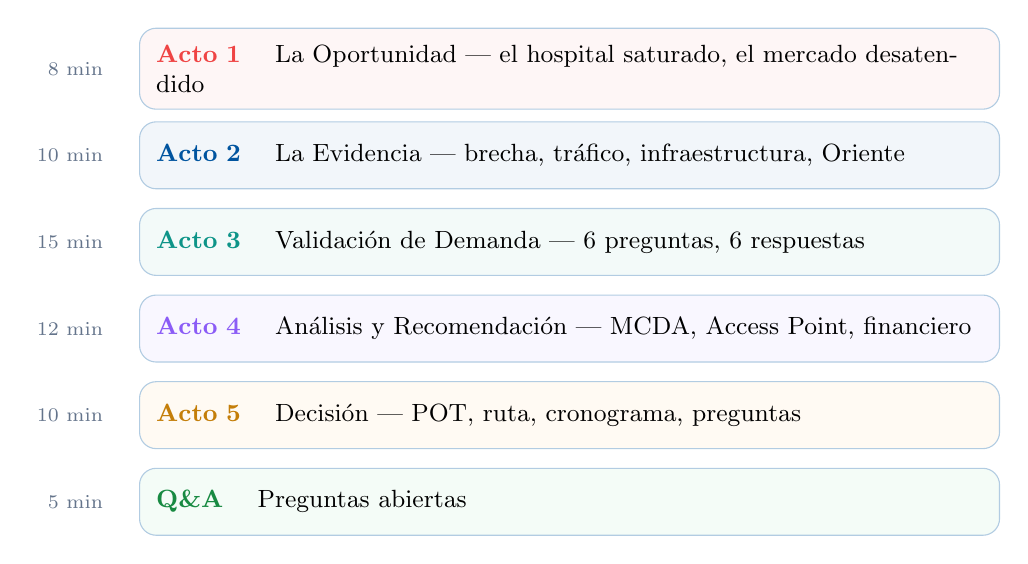
\begin{tikzpicture}[
  act/.style={draw=hptu!30, fill=white, rounded corners=6pt,
              text width=10.5cm, minimum height=0.85cm, align=left,
              font=\small, inner sep=6pt},
  time/.style={font=\scriptsize\color{slate}, anchor=east},
]
\node[act, fill=coral!5] (a1) at (0,0) {
  \textcolor{coral}{\textbf{Acto 1}} \quad La Oportunidad --- el hospital saturado, el mercado desatendido
};
\node[time] at (-5.8,0) {8 min};

\node[act, fill=hptu!5] (a2) at (0,-1.1) {
  \textcolor{hptu}{\textbf{Acto 2}} \quad La Evidencia --- brecha, tráfico, infraestructura, Oriente
};
\node[time] at (-5.8,-1.1) {10 min};

\node[act, fill=teal!5] (a3) at (0,-2.2) {
  \textcolor{teal}{\textbf{Acto 3}} \quad Validación de Demanda --- 6 preguntas, 6 respuestas
};
\node[time] at (-5.8,-2.2) {15 min};

\node[act, fill=violet!5] (a4) at (0,-3.3) {
  \textcolor{violet}{\textbf{Acto 4}} \quad Análisis y Recomendación --- MCDA, Access Point, financiero
};
\node[time] at (-5.8,-3.3) {12 min};

\node[act, fill=amber!5] (a5) at (0,-4.4) {
  \textcolor{amber!80!black}{\textbf{Acto 5}} \quad Decisión --- POT, ruta, cronograma, preguntas
};
\node[time] at (-5.8,-4.4) {10 min};

\node[act, fill=green!5] (q) at (0,-5.5) {
  \textcolor{green!70!black}{\textbf{Q\&A}} \quad Preguntas abiertas
};
\node[time] at (-5.8,-5.5) {5 min};
\end{tikzpicture}
\end{center}

\vspace{4pt}
{\footnotesize\textcolor{slate}{Plataforma interactiva: \url{https://hptu-localizacion.vercel.app}}}
\end{frame}

% ---- SLIDE 3: EL PROBLEMA ----
{
\setbeamercolor{background canvas}{bg=coral!3}
\begin{frame}{Un hospital saturado, lejos de su mercado}

\begin{columns}[T]
\column{0.52\textwidth}
\vspace{2pt}
\begin{center}
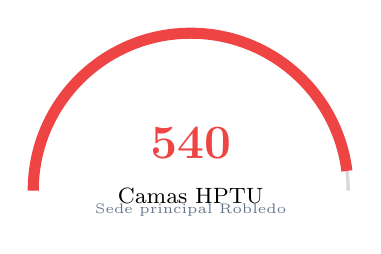
\begin{tikzpicture}
  \draw[gray!30, very thick] (0,0) arc (180:0:2);
  \draw[coral, line width=4pt] (0,0) arc (180:7.2:2);
  \node[font=\LARGE\bfseries, coral] at (2, 0.6) {540};
  \node[font=\footnotesize, below] at (2, 0.15) {Camas HPTU};
  \node[font=\tiny\color{slate}] at (2, -0.25) {Sede principal Robledo};
\end{tikzpicture}
\end{center}

\vspace{4pt}
{\small El HPTU opera en \textbf{Robledo} con 540 camas hospitalarias:}

\vspace{3pt}
\begin{itemize}\footnotesize
  \item \highlight{174,543 predios} E5/E6 en \textbf{22 barrios} del corredor
  \item A \danger{más de 20 minutos} del hospital
  \item Corredor Las Palmas: \danger{0 camas} de alta complejidad
  \item \highlight{103,913 hab.} sin cobertura a 2037
\end{itemize}

\column{0.45\textwidth}
\begin{alertblock}{\small El déficit es real}
\footnotesize
La OMS recomienda \textbf{3--5 camas} por cada 1,000 habitantes.

\vspace{4pt}
\begin{tabular}{@{}lc@{}}
\toprule
\textbf{Municipio} & \textbf{Camas/1000} \\
\midrule
\rowcolor{coral!10}
Medellín & \danger{1.0} \\
\rowcolor{coral!8}
Envigado & \danger{0.6} \\
Itagüí & \danger{0.6} \\
Sabaneta & \danger{0.5} \\
\midrule
\textbf{OMS mínimo} & \highlight{3.0} \\
\bottomrule
\end{tabular}
\end{alertblock}

\vspace{6pt}
\begin{exampleblock}{\small Nos preguntamos}
\centering\normalsize
\textbf{¿Dónde debe estar\\la nueva sede?}
\end{exampleblock}
\end{columns}
\end{frame}
}

% ---- SLIDE 4: LA ESCALA DEL ANÁLISIS ----
\begin{frame}{La escala del análisis: datos, no opiniones}

\vspace{-2pt}
\begin{center}
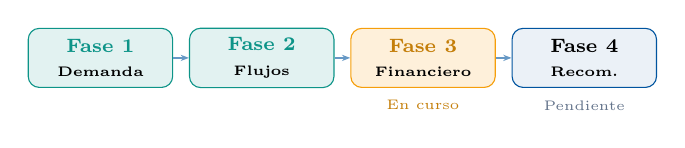
\begin{tikzpicture}[
  node distance=0.2cm,
  phase/.style={draw=hptu, fill=hptu!8, rounded corners=4pt,
                text width=1.6cm, minimum height=0.75cm, align=center,
                font=\scriptsize\bfseries},
  done/.style={phase, fill=teal!12, draw=teal},
  active/.style={phase, fill=amber!15, draw=amber},
  arrow/.style={-{Stealth[length=3pt]}, thick, hptu!60}
]
\node[done] (p1) {\textcolor{teal}{Fase 1}\\[1pt]\tiny Demanda};
\node[done, right=of p1] (p2) {\textcolor{teal}{Fase 2}\\[1pt]\tiny Flujos};
\node[active, right=of p2] (p3) {\textcolor{amber!80!black}{Fase 3}\\[1pt]\tiny Financiero};
\node[phase, right=of p3] (p4) {Fase 4\\[1pt]\tiny Recom.};

\draw[arrow] (p1) -- (p2);
\draw[arrow] (p2) -- (p3);
\draw[arrow] (p3) -- (p4);

\node[below=1pt of p1, font=\tiny\color{teal}] {\checkmark};
\node[below=1pt of p2, font=\tiny\color{teal}] {\checkmark};
\node[below=1pt of p3, font=\tiny\color{amber!80!black}] {En curso};
\node[below=1pt of p4, font=\tiny\color{slate}] {Pendiente};
\end{tikzpicture}
\end{center}

\vspace{2pt}
\begin{columns}[T]
\column{0.48\textwidth}
\begin{block}{\small Escala del análisis}
\scriptsize
\begin{tabular}{@{}lr@{}}
\toprule
Fuentes primarias & \textbf{15} \\
Registros procesados & \textbf{3.8M+} \\
Zonas evaluadas & \textbf{6} \\
Competidores perfilados & \textbf{13} \\
IPS georreferenciadas & \textbf{145} \\
Barrios analizados & \textbf{22} \\
Variables DENSURBAM & \textbf{59} \\
Periodo de datos & 2017--2037 \\
\bottomrule
\end{tabular}
\end{block}

\column{0.48\textwidth}
\begin{exampleblock}{\small Modelo MCDA (score 0--100)}
\scriptsize
Cada zona se evalúa en 4 dimensiones:

\vspace{3pt}
$\text{Score} = \underbrace{A \times 35\%}_{\text{Acc.}} + \underbrace{D \times 30\%}_{\text{Dem.}} + \underbrace{C \times 20\%}_{\text{Comp.}} + \underbrace{V \times 15\%}_{\text{Val.Inm.}}$

\vspace{4pt}
Sensibilidad validada con \textbf{Monte Carlo} (3,000 iteraciones). Recomendación final pondera score + posición estratégica.
\end{exampleblock}
\end{columns}

\vspace{2pt}
{\scriptsize\color{slate} Fuentes: Catastro, REPS, MEData, DANE, POT, ProColombia, ANI, BDUA, Mapbox, Google Places.}
\end{frame}

% ---- SLIDE 5: EL MERCADO OBJETIVO ----
\begin{frame}{El mercado: 174,543 predios E5/E6 en 22 barrios}

\begin{columns}[T]
\column{0.46\textwidth}
\vspace{-2pt}
{\scriptsize\setlength{\tabcolsep}{3pt}
\begin{tabular}{@{}lrrc@{}}
\toprule
\textbf{Barrio} & \textbf{E5/E6} & \textbf{\%} & \textbf{Avalúo} \\
\midrule
\rowcolor{teal!8}
\textbf{El Poblado core} & \textbf{38,415} & \textbf{98} & \$371M \\
Castropol & 6,228 & 97 & \$327M \\
Los Balsos No.\ 1 & 4,019 & 95 & \$401M \\
San Lucas & 3,671 & 93 & \$512M \\
Manila & 2,144 & 96 & \$305M \\
\rowcolor{teal!6}
Altos del Poblado & 1,867 & 91 & \$245M \\
El Tesoro & 1,856 & 89 & \$258M \\
{\tiny + 15 barrios más} & & & \\
\midrule
\textbf{Total 22 barrios} & \textbf{174,543} & & \\
\bottomrule
\end{tabular}
}

\vspace{3pt}
\src{Catastro Municipal Medellín (bp59-rj8r), 1,041,413 predios}

\column{0.50\textwidth}
\vspace{-2pt}
\begin{exampleblock}{\small Perfil del mercado}
\scriptsize
\begin{itemize}\setlength{\itemsep}{0pt}\setlength{\parskip}{0pt}
  \item \textbf{Prepagada}: SURA con \highlight{320,000 afiliados} en El Poblado
  \item \textbf{Colegios}: Colombo Británico, Montessori --- 30 instit.
  \item \textbf{Clubes}: El Rodeo, Campestre Medellín
  \item \textbf{Corporativo}: Milla de Oro, Bancolombia (4,000 emp.)
\end{itemize}
\end{exampleblock}

\vspace{2pt}
\begin{alertblock}{\small 0 camas para este mercado}
\scriptsize Ningún hospital en el corredor ofrece trasplantes, hematología ni oncología. HPTU sería el \textbf{único} de alta complejidad.
\end{alertblock}

\vspace{2pt}
{\scriptsize Corredor Las Palmas: \textbf{88--98\%} E5/E6, avalúos \highlight{\$245M--\$512M COP}.}
\end{columns}
\end{frame}

% ============================================================
% ACTO 2: LA EVIDENCIA (slides 6--10, ~10 min)
% ============================================================

% ---- SLIDE 6: LA BRECHA ----
{
\setbeamercolor{background canvas}{bg=coral!3}
\begin{frame}{La brecha: un corredor sin hospital de alta complejidad}

\begin{columns}[T]
\column{0.48\textwidth}
\textbf{DENSURBAM confirma} (Variable 49 --- IRS Salud):

\vspace{4pt}
\begin{center}
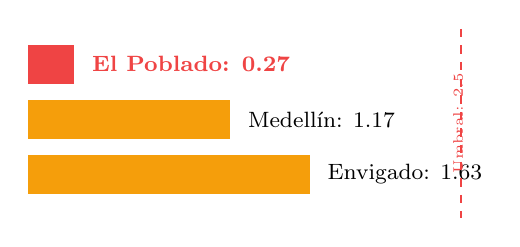
\begin{tikzpicture}
  \fill[coral] (0,0) rectangle (0.27/2.5*5.5, 0.5);
  \node[right, font=\footnotesize\bfseries] at (0.27/2.5*5.5+0.1, 0.25) {\danger{El Poblado: 0.27}};

  \fill[amber] (0,-0.7) rectangle (1.17/2.5*5.5, -0.2);
  \node[right, font=\footnotesize] at (1.17/2.5*5.5+0.1, -0.45) {Medellín: 1.17};

  \fill[amber] (0,-1.4) rectangle (1.63/2.5*5.5, -0.9);
  \node[right, font=\footnotesize] at (1.63/2.5*5.5+0.1, -1.15) {Envigado: 1.63};

  \draw[coral, thick, dashed] (2.5/2.5*5.5, 0.7) -- (2.5/2.5*5.5, -1.7);
  \node[font=\tiny, coral, rotate=90, anchor=south] at (2.5/2.5*5.5+0.15, -0.5) {Umbral: 2.5};
\end{tikzpicture}
\end{center}

\vspace{4pt}
\textbf{10 barrios} del corredor tienen \danger{0.0 m²} de oferta de salud.

\vspace{4pt}
{\footnotesize IRS = Índice de Redistribución de Salud. El Poblado tiene \danger{5 veces menos} infraestructura que el promedio de Medellín.}

\src{DENSURBAM (URBAM-EAFIT/AMVA), 59 variables}

\column{0.49\textwidth}
\textbf{Red hospitalaria actual}:

\vspace{4pt}
{\scriptsize
\begin{tabular}{@{}lrl@{}}
\toprule
\textbf{Hospital} & \textbf{Camas} & \textbf{Dist.} \\
\midrule
\rowcolor{coral!10}
HPTU Robledo & 540 & 8.5 km \\
Cl.\ Medellín & 184 & 3.2 km \\
HGM ESE & 384 & 7+ km \\
Cl.\ del Prado & 152 & 5+ km \\
Cl.\ CES & 213 & 7.16 km \\
H.\ Uribe Ángel & 120 & Envigado \\
\midrule
\textbf{Total sistema} & \textbf{1,593} & \\
\bottomrule
\end{tabular}
}

\vspace{6pt}
\begin{alertblock}{\small En el corredor Las Palmas}
\footnotesize
\begin{tabular}{@{}lcc@{}}
Cl.\ Rosario Tesoro & 158 camas & sin trasplantes \\
Cl.\ Las Vegas & 171 camas & sin oncología \\
\end{tabular}

\vspace{3pt}
\danger{0 camas} de alta complejidad.
\end{alertblock}
\end{columns}
\end{frame}
}

% ---- SLIDE 7: PROYECCIÓN 2037 — VALLE + ORIENTE ----
\begin{frame}{Proyección 2037: crecimiento en dos frentes}

\begin{columns}[T]
\column{0.48\textwidth}
{\small\textbf{Valle de Aburrá} (DENSURBAM):}

\vspace{3pt}
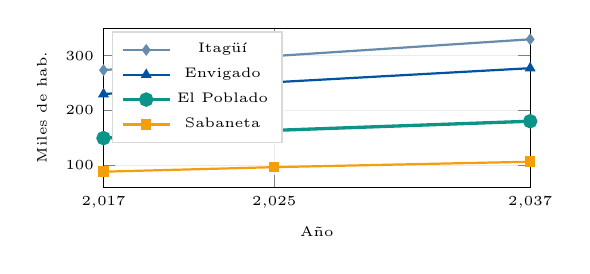
\begin{tikzpicture}
\begin{axis}[
  width=7cm, height=3.6cm,
  xlabel={\tiny Año},
  ylabel={\tiny Miles de hab.},
  xmin=2017, xmax=2037, ymin=60, ymax=350,
  xtick={2017,2025,2037},
  xticklabel style={font=\tiny},
  yticklabel style={font=\tiny},
  grid=major, grid style={gray!15},
  legend style={at={(0.02,0.98)}, anchor=north west, font=\tiny,
               fill=white, draw=gray!30},
]
\addplot[hptudark!60, thick, mark=diamond*, mark size=1.5pt] coordinates {
  (2017,273.5)(2025,299.2)(2037,329.8)
};
\addlegendentry{Itagüí}
\addplot[hptu, thick, mark=triangle*, mark size=1.5pt] coordinates {
  (2017,229.8)(2025,251.4)(2037,277.1)
};
\addlegendentry{Envigado}
\addplot[teal, very thick, mark=*, mark size=2pt] coordinates {
  (2017,149.5)(2025,163.6)(2037,180.3)
};
\addlegendentry{El Poblado}
\addplot[amber, thick, mark=square*, mark size=1.5pt] coordinates {
  (2017,88.2)(2025,96.5)(2037,106.4)
};
\addlegendentry{Sabaneta}
\end{axis}
\end{tikzpicture}

{\tiny Valle de Aburrá: \textbf{+152K} personas a 2037. Fuente: DENSURBAM (DANE + AMVA).}

\vspace{4pt}
\begin{alertblock}{\small La ecuación}
\scriptsize
Red de \danger{1,593 camas} para 2.5M+ hab.\\
\textbf{+ 152K Valle + crecimiento Oriente}\\
\textbf{+ 0 camas nuevas en el corredor}\\[2pt]
{\color{coral}\rule{\textwidth}{0.4pt}}\\[2pt]
= Infraestructura requerida: \danger{363,696 m²}
\end{alertblock}

\column{0.49\textwidth}
{\small\textbf{Oriente Antioqueño} (DANE + DNP):}

\vspace{3pt}
{\scriptsize
\begin{tabular}{@{}lrrr@{}}
\toprule
\textbf{Municipio} & \textbf{2018} & \textbf{2026} & \textbf{CAGR} \\
\midrule
\rowcolor{teal!8}
\textbf{Rionegro} & 116K & \highlight{138K} & \highlight{+2.0\%} \\
La Ceja & 59K & 69K & +1.9\% \\
Marinilla & 55K & 64K & +1.9\% \\
El Carmen & 54K & 63K & +1.9\% \\
Guarne & 43K & 49K & +1.7\% \\
El Santuario & 30K & 35K & +2.0\% \\
El Retiro & 21K & 24K & +1.7\% \\
\midrule
\rowcolor{teal!6}
\textbf{7 municipios} & \textbf{378K} & \textbf{442K} & \\
\bottomrule
\end{tabular}
}

\vspace{4pt}
\begin{exampleblock}{\small El Oriente crece al doble}
\scriptsize
Rionegro: \highlight{+2.0\%} anual vs Medellín \textbf{+0.9\%}.

\vspace{2pt}
Proyección Rionegro 2030: \highlight{149K hab}.

\vspace{2pt}
Tasa migración neta: \textbf{5.2/100 hab/año} --- el Oriente atrae población.
\end{exampleblock}

\vspace{2pt}
\src{DANE CNPV 2018 (evm3-92yw), DNP Proyecciones}
\end{columns}
\end{frame}

% ---- SLIDE 8: EL TRÁFICO ----
\begin{frame}{El tráfico: Las Palmas fluye, El Poblado colapsa}

\begin{columns}[T]
\column{0.50\textwidth}
Con \highlight{682,502 observaciones} de MEData (2017--2020):

\vspace{4pt}
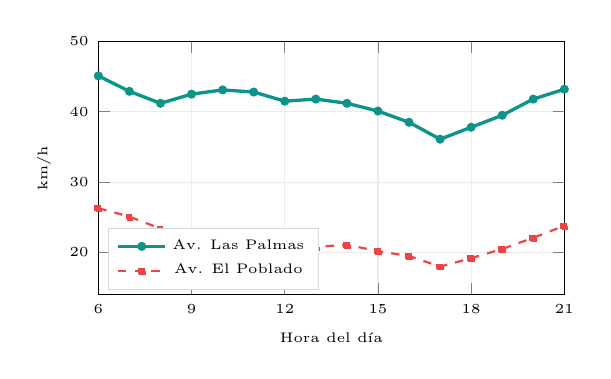
\begin{tikzpicture}
\begin{axis}[
  width=7.5cm, height=4.8cm,
  xlabel={\tiny Hora del día},
  ylabel={\tiny km/h},
  xmin=6, xmax=21, ymin=14, ymax=50,
  xtick={6,9,12,15,18,21},
  xticklabel style={font=\tiny},
  yticklabel style={font=\tiny},
  grid=major, grid style={gray!15},
  legend style={at={(0.02,0.02)}, anchor=south west, font=\tiny,
               fill=white, draw=gray!30},
]
\addplot[teal, very thick, mark=*, mark size=1pt] coordinates {
  (6,45.1)(7,42.9)(8,41.2)(9,42.5)(10,43.1)(11,42.8)
  (12,41.5)(13,41.8)(14,41.2)(15,40.1)(16,38.5)(17,36.1)
  (18,37.8)(19,39.5)(20,41.8)(21,43.2)
};
\addlegendentry{Av. Las Palmas}
\addplot[coral, thick, dashed, mark=square*, mark size=1pt] coordinates {
  (6,26.3)(7,25.1)(8,23.4)(9,22.8)(10,21.9)(11,21.2)
  (12,20.5)(13,20.8)(14,21.1)(15,20.2)(16,19.5)(17,18.0)
  (18,19.2)(19,20.5)(20,22.1)(21,23.8)
};
\addlegendentry{Av. El Poblado}
\end{axis}
\end{tikzpicture}

\src{MEData Velocidad Tiempo Viaje GT (7t5n-3b3w)}

\column{0.47\textwidth}
\vspace{8pt}
A las \textbf{5:00 PM} (hora pico):

\vspace{4pt}
\begin{alertblock}{}
\centering
{\Large \danger{18.0 km/h}}\\
\footnotesize Av.\ El Poblado --- congestión severa
\end{alertblock}

\vspace{2pt}
\begin{exampleblock}{}
\centering
{\Large \highlight{40.9 km/h}}\\
\footnotesize Av.\ Las Palmas --- \textbf{100\% más rápido}
\end{exampleblock}

\vspace{6pt}
{\footnotesize\textbf{Desde 6 orígenes} a Las Palmas Bajo:}

\vspace{3pt}
{\scriptsize
\begin{tabular}{@{}lrl@{}}
Milla de Oro & \highlight{15.4 min} & \\
El Poblado & \highlight{17.7 min} & \\
Envigado & 24.8 min & \\
Laureles & 32.3 min & \\
\midrule
\textbf{Promedio} & \textbf{26.6 min} & \\
\end{tabular}
}
\end{columns}
\end{frame}

% ---- SLIDE 9: INFRAESTRUCTURA VIAL ----
\begin{frame}{Infraestructura vial: COP \$1.96 billones en camino}

{\tiny
\begin{tabular}{@{}p{3.0cm}rlcp{4.5cm}@{}}
\toprule
\textbf{Proyecto} & \textbf{Inversión} & \textbf{Status} & \textbf{Timeline} & \textbf{Impacto en Km 7} \\
\midrule
\rowcolor{teal!8}
2da Etapa Túnel Oriente & \$1.8 bill. & Construcción & H2 2027 & \highlight{CRÍTICO}: doble calzada, Km 7 nodo de entrada \\
Intercambio Alto Palmas & \$18,000M & Planeado & Q2 2026 & DIRECTO: elimina congestión aguas arriba \\
Vía Aeropuerto-Belén & \$120,000M & Planeado & Q2 2026 & ALTO: circuito hospital-aeropuerto \\
Vía Llanogrande-Cañada & \$120,000M & Planeado & 2026+ & ALTO: alimenta tráfico corredor túnel \\
Doble calzada Ceja-Rionegro & N/D & Construcción & Mar 2026 & MEDIO: flujo intra-Oriente \\
\bottomrule
\end{tabular}
}

\vspace{8pt}
\begin{columns}[T]
\column{0.48\textwidth}
\begin{exampleblock}{\small Convergencia vial en Km 7}
\footnotesize
\begin{enumerate}
  \item Túnel doble calzada (H2 2027) = \textbf{Rionegro a 25 min}
  \item Intercambio Alto Palmas = \textbf{cero congestión}
  \item Vía Aeropuerto = \textbf{circuito completo}
\end{enumerate}

\vspace{3pt}
Km 7 queda en la \textbf{intersección de las 3 obras}.
\end{exampleblock}

\column{0.48\textwidth}
\begin{block}{\small Otros proyectos en evaluación}
\footnotesize
\begin{itemize}
  \item Tren Medellín-Oriente: estudios (\$3,421M)
  \item Tren Ligero Rionegro: \danger{anulado} (fallo judicial)
  \item Vía Santa Elena: mejoramiento (\$5,500M)
\end{itemize}
\end{block}
\end{columns}

\src{ANI, INVIAS, Gobernación de Antioquia, Plan Maestro JMC 2055}
\end{frame}

% ---- SLIDE 10: EL ORIENTE CRECE ----
{
\setbeamercolor{background canvas}{bg=teal!3}
\begin{frame}{El Oriente crece: la demanda viene hacia nosotros}

\begin{columns}[T]
\column{0.48\textwidth}
\begin{center}
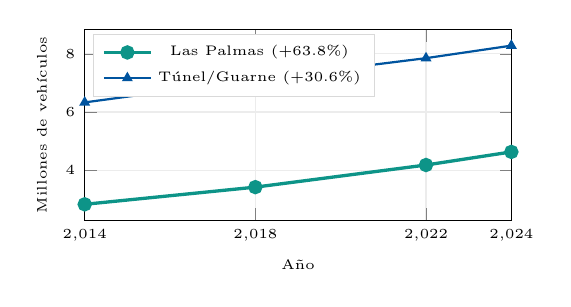
\begin{tikzpicture}
\begin{axis}[
  width=7cm, height=4cm,
  xlabel={\tiny Año},
  ylabel={\tiny Millones de vehículos},
  xmin=2014, xmax=2024,
  xtick={2014,2018,2022,2024},
  xticklabel style={font=\tiny},
  yticklabel style={font=\tiny},
  grid=major, grid style={gray!15},
  legend style={at={(0.02,0.98)}, anchor=north west, font=\tiny,
               fill=white, draw=gray!30},
]
\addplot[teal, very thick, mark=*, mark size=2pt] coordinates {
  (2014,2.83)(2018,3.42)(2022,4.18)(2024,4.63)
};
\addlegendentry{Las Palmas (+63.8\%)}
\addplot[hptu, thick, mark=triangle*, mark size=1.5pt] coordinates {
  (2014,6.33)(2018,7.12)(2022,7.85)(2024,8.28)
};
\addlegendentry{Túnel/Guarne (+30.6\%)}
\end{axis}
\end{tikzpicture}
\end{center}

\src{ANI peajes (8yi9-t44c), 2014--2024 exactos}

\vspace{4pt}
{\footnotesize Tráfico Las Palmas: de 2.8M a 4.6M veh/año. \textbf{+63.8\% en 10 años.} La demanda de servicios de salud sigue al tráfico.}

\column{0.49\textwidth}
\vspace{4pt}
{\small 4 señales de crecimiento:}

\vspace{4pt}
{\scriptsize
\begin{tabular}{@{}p{3.2cm}rl@{}}
\toprule
\textbf{Indicador} & \textbf{Valor} & \textbf{Trend} \\
\midrule
\rowcolor{teal!6}
Rionegro CAGR & \highlight{+2.0\%} & $\uparrow$ \\
Tráfico Las Palmas & \highlight{+63.8\%} & $\uparrow$ \\
Aeropuerto JMC & 14.5M $\to$ 42.7M & $\uparrow$ \\
\rowcolor{teal!6}
Migración Oriente & 5.2/100 hab & $\uparrow$ \\
Prepagada Antioquia & +37\% (2022-25) & $\uparrow$ \\
Turismo médico & +15\% CAGR & $\uparrow$ \\
2da etapa Túnel & H2 2027 & $\uparrow$ \\
PIB Oriente/Antioquia & 10.4\% & $\uparrow$ \\
\bottomrule
\end{tabular}
}

\vspace{6pt}
\begin{exampleblock}{\small La evidencia muestra}
\footnotesize \textbf{8 de 8 indicadores} apuntan hacia arriba. No es una apuesta --- es una tendencia consolidada.
\end{exampleblock}
\end{columns}
\end{frame}
}

% ---- SLIDE 11: ORIENTE — INFRAESTRUCTURA DE SALUD ----
{
\setbeamercolor{background canvas}{bg=coral!3}
\begin{frame}{Oriente Antioqueño: 728,000 habitantes, infraestructura crítica}

\begin{columns}[T]
\column{0.48\textwidth}
\vspace{2pt}
{\small\textbf{Infraestructura de salud} (11 municipios):}

\vspace{4pt}
{\scriptsize
\begin{tabular}{@{}lrrr@{}}
\toprule
\textbf{Municipio} & \textbf{Camas} & \textbf{/1000} & \textbf{Gap OMS} \\
\midrule
\rowcolor{teal!6}
Rionegro & 656 & 4.86 & --- \\
La Ceja & 240 & 3.48 & --- \\
Guarne & 184 & 3.73 & --- \\
\rowcolor{coral!10}
El Carmen & 37 & \danger{0.59} & +1.91 \\
\rowcolor{coral!10}
Marinilla & 27 & \danger{0.42} & +2.08 \\
\rowcolor{coral!10}
El Retiro & 26 & \danger{1.08} & +1.42 \\
\rowcolor{coral!10}
El Santuario & 6 & \danger{0.17} & +2.33 \\
\midrule
\textbf{Total Oriente} & \textbf{1,199} & & \\
\bottomrule
\end{tabular}
}

\vspace{4pt}
\src{REPS capacidad instalada (b4dp-ximh), DANE est.\ 2026}

\column{0.49\textwidth}
\vspace{2pt}
\begin{alertblock}{\small 3 datos críticos del Oriente}
\footnotesize
\begin{enumerate}\setlength{\itemsep}{0pt}\setlength{\parskip}{0pt}
  \item \textbf{55\%} de las camas concentradas en Rionegro
  \item \danger{0 hospitales} nivel 3--4 en toda la región
  \item \textbf{4 municipios} con menos de 1 cama/1000 hab
\end{enumerate}

\vspace{4pt}
Solo \textbf{Cl.\ Somer} ofrece oncología (única UFCA) y radioterapia (único equipo) en todo el Oriente.
\end{alertblock}

\vspace{4pt}
\begin{exampleblock}{\small Mercado contributivo Oriente}
\scriptsize
\begin{tabular}{@{}lr@{}}
Afiliados contributivos & \highlight{384,171} \\
Ratio C/S & \highlight{3.46$\times$} \\
Rionegro \% contributivo & \highlight{85\%} \\
SURA dominancia & 64--79\% del mercado \\
Prepagada Antioquia & +37\% (2022--2025) \\
Zona Franca & 300+ empresas, 12K emp. \\
\end{tabular}

\vspace{2pt}
{\tiny Fuente: BDUA marzo 2026 (ADRES)}
\end{exampleblock}
\end{columns}
\end{frame}
}

% ---- SLIDE 12: ORIENTE — DEMANDA CAPTURABLE ----
\begin{frame}{Demanda capturable: 45,000 consultas/año desde el Oriente}

\begin{columns}[T]
\column{0.50\textwidth}
\vspace{2pt}
{\small\textbf{Flujo de pacientes Oriente $\to$ Medellín}:}

\vspace{4pt}
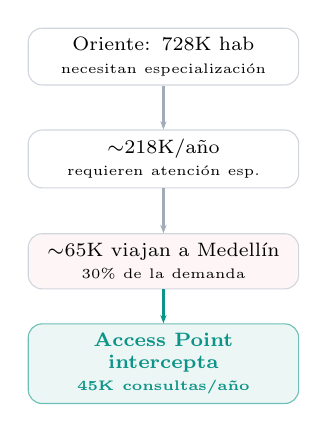
\begin{tikzpicture}[
  box/.style={draw=slate!30, fill=white, rounded corners=5pt,
              text width=3.2cm, minimum height=0.7cm, align=center,
              font=\scriptsize},
  hub/.style={box, draw=teal!60, fill=teal!8, font=\scriptsize\bfseries},
  flow/.style={-{Stealth[length=3pt]}, thick},
]
\node[box] (pop) at (0,0) {Oriente: 728K hab\\{\tiny necesitan especialización}};
\node[box] (need) at (0,-1.3) {$\sim$218K/año\\{\tiny requieren atención esp.}};
\node[box, fill=coral!5] (med) at (0,-2.6) {$\sim$65K viajan a Medellín\\{\tiny 30\% de la demanda}};
\node[hub] (ap) at (0,-3.9) {\textcolor{teal}{Access Point intercepta}\\{\tiny \highlight{45K consultas/año}}};

\draw[flow, slate!60] (pop) -- (need);
\draw[flow, slate!60] (need) -- (med);
\draw[flow, teal] (med) -- (ap);
\end{tikzpicture}

\vspace{4pt}
\src{REPS, SISPRO 2023, modelo de demanda ambulatoria}

\column{0.47\textwidth}
\vspace{2pt}
{\small\textbf{Portafolio capturable}:}

\vspace{4pt}
{\scriptsize
\begin{tabular}{@{}lrr@{}}
\toprule
\textbf{Servicio} & \textbf{Vol./año} & \textbf{Revenue} \\
\midrule
\rowcolor{teal!6}
Consulta especializada & 18,000 & \$3,240M \\
Cirugía ambulatoria & 6,500 & \$2,600M \\
\rowcolor{teal!6}
Imágenes diagnósticas & 9,000 & \$1,350M \\
Rehabilitación & 7,000 & \$560M \\
\rowcolor{teal!6}
Chequeo ejecutivo & 4,500 & \$350M \\
\midrule
\textbf{TOTAL} & \textbf{45,000} & \highlight{\$8,100M} \\
\bottomrule
\end{tabular}
}

\vspace{6pt}
\begin{exampleblock}{\small Por qué Access Point intercepta}
\scriptsize
\begin{itemize}\setlength{\itemsep}{0pt}\setlength{\parskip}{0pt}
  \item \textbf{--17.8 min} vs HPTU a El Retiro y La Ceja
  \item Nodo de entrada del \textbf{Túnel} (H2 2027)
  \item \textbf{40--46\%} de pacientes Rionegro son no residentes
  \item Zona Franca: 12K empleados sin chequeo ejecutivo
\end{itemize}
\end{exampleblock}
\end{columns}
\end{frame}

% ---- SLIDE 13: ORIENTE — BRECHAS AMBULATORIAS ----
{
\setbeamercolor{background canvas}{bg=coral!3}
\begin{frame}{Oriente: 5 servicios críticos, 4 inexistentes}

\vspace{-2pt}
{\scriptsize\setlength{\tabcolsep}{3pt}
\begin{tabular}{@{}p{3.0cm}p{3.2cm}lp{4.0cm}@{}}
\toprule
\textbf{Servicio} & \textbf{Status Oriente} & \textbf{Nivel} & \textbf{Oportunidad HPTU} \\
\midrule
\rowcolor{coral!10}
Cirugía Ambulat.\ Avanzada & Solo Campestre (recién) & \danger{Crítico} & Hub quirúrgico especializado \\
\rowcolor{coral!10}
Oncología Ambulatoria & Solo Somer (única UFCA) & \danger{Crítico} & Quimioterapia, 2da opinión \\
\rowcolor{coral!10}
Radioterapia & Solo Somer (único equipo) & \danger{Crítico} & 2do centro para la región \\
Imágenes Avanzadas & IMEDI + Somer (limitado) & Limitado & TAC, RMN, PET-CT \\
\rowcolor{coral!6}
Rehabilitación Especial. & Básica únicamente & \danger{Inexist.} & Neuro-rehab, cardíaca, deportiva \\
\rowcolor{coral!6}
Chequeo Ejecutivo & Inexistente & \danger{Inexist.} & Check-up Zona Franca + aerop. \\
\rowcolor{coral!6}
Turismo Médico & 0 infraestructura & \danger{Inexist.} & 0 JCI cerca de SKRG \\
\rowcolor{coral!6}
Pediatría Subespec. & Solo en Medellín & \danger{Inexist.} & Consulta ped.\ ambulatoria \\
Hemodiálisis & RCS Rionegro (41\%) & Limitado & Expansión puntos diálisis \\
\bottomrule
\end{tabular}
}

\vspace{6pt}
\begin{columns}[T]
\column{0.48\textwidth}
\begin{alertblock}{\small Monopolios en el Oriente}
\scriptsize
Somer tiene el \textbf{único equipo de radioterapia} y la \textbf{única UFCA} (oncología). Un solo proveedor para 728K habitantes. HPTU rompería ese monopolio con calidad JCI.
\end{alertblock}

\column{0.48\textwidth}
\begin{exampleblock}{\small El Oriente necesita}
\scriptsize
\textbf{3 servicios críticos + 4 inexistentes} = oportunidad masiva para hub ambulatorio especializado que ningún competidor actual puede ofrecer con calidad HPTU.
\end{exampleblock}
\end{columns}
\end{frame}
}

% ============================================================
% ACTO 3: VALIDACIÓN DE DEMANDA — 6 PREGUNTAS
% ============================================================

% ---- SLIDE ~: DIVIDER ----
{
\setbeamercolor{background canvas}{bg=hptu}
\begin{frame}[plain]
\vfill
\begin{center}
{\Huge\bfseries\textcolor{white}{Las 6 preguntas\\[8pt]que la Junta\\[8pt]necesita responder}}

\vspace{20pt}
\begin{tikzpicture}
  \draw[white, line width=0.5pt] (0,0) -- (8,0);
\end{tikzpicture}

\vspace{14pt}
{\normalsize\textcolor{white!80}{Validación de demanda basada en evidencia}}
\end{center}
\vfill
\end{frame}
}

% ---- SLIDE 12: Q1 ----
{
\setbeamercolor{background canvas}{bg=coral!3}
\begin{frame}{Q1: ¿Hay suficientes pacientes?}

\begin{columns}[T]
\column{0.50\textwidth}
\vspace{4pt}
{\small\textbf{Brecha de oferta en el Oriente} (7 municipios):}

\vspace{4pt}
{\scriptsize
\begin{tabular}{@{}lrrr@{}}
\toprule
\textbf{Municipio} & \textbf{Camas} & \textbf{Camas/1000} & \textbf{Gap OMS} \\
\midrule
\rowcolor{coral!6}
Rionegro & 656 & 4.86 & -- \\
La Ceja & 240 & 3.48 & -- \\
Guarne & 184 & 3.73 & -- \\
\rowcolor{coral!12}
El Carmen & 37 & \danger{0.59} & +1.91 \\
\rowcolor{coral!12}
Marinilla & 27 & \danger{0.42} & +2.08 \\
\rowcolor{coral!12}
El Retiro & 26 & \danger{1.08} & +1.42 \\
\rowcolor{coral!12}
El Santuario & 6 & \danger{0.17} & +2.33 \\
\bottomrule
\end{tabular}
}

\vspace{4pt}
\src{REPS capacidad instalada (b4dp-ximh), DANE est. 2026}

\column{0.47\textwidth}
\vspace{4pt}
\begin{alertblock}{\small Los 3 datos que importan}
\footnotesize
\begin{enumerate}
  \item Rionegro: \danger{0 camas UCI} en 2023 (bajó de 0.14/1000)
  \item Sobreocupación: \danger{114\%} en urgencias
  \item \textbf{40--46\%} de pacientes en Rionegro son \textbf{no residentes} ($\sim$33,600/año)
\end{enumerate}

\vspace{4pt}
Los pacientes \textbf{ya están viajando}. La pregunta no es si hay demanda --- es quién la captura.
\end{alertblock}

\vspace{4pt}
\begin{exampleblock}{\small Respuesta}
\centering\large
\highlight{Sí. Sobran.}
\end{exampleblock}
\end{columns}
\end{frame}
}

% ---- SLIDE 13: Q2 ----
\begin{frame}{Q2: ¿Vendrán a Km 7?}

\begin{columns}[T]
\column{0.52\textwidth}
\vspace{2pt}
{\small Tiempos de viaje: \textbf{Km 7 vs HPTU} (hoy + post Túnel H2 2027):}

\vspace{4pt}
{\scriptsize
\begin{tabular}{@{}lcccl@{}}
\toprule
\textbf{Destino} & \textbf{Km 7} & \textbf{Post Túnel} & \textbf{HPTU} & \textbf{Ahorro} \\
\midrule
\rowcolor{teal!10}
Aeropuerto & 51' & \highlight{25'} & 66' & \highlight{--41'} \\
\rowcolor{teal!10}
Rionegro & 59' & \highlight{25'} & 57' & \highlight{--32'} \\
\rowcolor{teal!10}
El Retiro & 44' & \highlight{30'} & 62' & \highlight{--32'} \\
\rowcolor{teal!10}
La Ceja & 66' & \highlight{40'} & 84' & \highlight{--44'} \\
Guarne & 56' & $\sim$40' & 40' & $\sim$similar \\
Marinilla & 68' & $\sim$45' & 59' & \highlight{--14'} \\
\bottomrule
\end{tabular}
}

\vspace{3pt}
{\tiny Hoy: Mapbox Matrix API. Post Túnel: estimación con doble calzada H2 2027 (Rionegro a 25 min desde Km 7).}

\vspace{3pt}
\src{Mapbox Matrix API, ANI/INVIAS proyección Túnel 2da etapa}

\column{0.45\textwidth}
\vspace{2pt}
\begin{exampleblock}{\small Post Túnel: Km 7 gana en todo}
\footnotesize
Con la doble calzada (H2 2027), Km 7 se convierte en el \textbf{nodo de entrada}:

\vspace{3pt}
\begin{itemize}
  \item \textbf{Aeropuerto}: \highlight{25 min} (vs HPTU 66')
  \item \textbf{Rionegro}: \highlight{25 min} (vs HPTU 57')
  \item \textbf{El Retiro}: \highlight{30 min} (vs HPTU 62')
  \item \textbf{La Ceja}: \highlight{40 min} (vs HPTU 84')
\end{itemize}

\vspace{3pt}
Km 7 pasa de ganar en \textbf{3 de 7} destinos a ganar en \textbf{6 de 6}.
\end{exampleblock}

\vspace{4pt}
\begin{exampleblock}{\small Respuesta}
\centering\large
\highlight{Sí. 6 de 6 post Túnel.}
\end{exampleblock}
\end{columns}
\end{frame}

% ---- SLIDE 14: Q3 ----
\begin{frame}{Q3: ¿Pueden pagar?}

\begin{columns}[T]
\column{0.50\textwidth}
\vspace{4pt}
{\small\textbf{Afiliación EPS en el catchment} (7 municipios, BDUA Mar 2026):}

\vspace{4pt}
{\scriptsize
\begin{tabular}{@{}lrrc@{}}
\toprule
\textbf{Municipio} & \textbf{Contrib.} & \textbf{Total} & \textbf{\%C} \\
\midrule
\rowcolor{teal!8}
Rionegro & 169,749 & 199,690 & \highlight{85\%} \\
La Ceja & 64,947 & 78,176 & 83\% \\
Marinilla & 47,398 & 67,067 & 71\% \\
El Carmen & 35,869 & 52,179 & 69\% \\
Guarne & 35,698 & 48,355 & 74\% \\
El Retiro & 15,530 & 19,268 & \highlight{81\%} \\
El Santuario & 14,980 & 30,492 & 49\% \\
\midrule
\rowcolor{teal!10}
\textbf{TOTAL} & \textbf{384,171} & \textbf{495,227} & \textbf{78\%} \\
\bottomrule
\end{tabular}
}

\src{BDUA marzo 2026 (ADRES)}

\column{0.47\textwidth}
\vspace{4pt}
\begin{exampleblock}{\small 3 indicadores clave}
\footnotesize
\begin{tabular}{@{}lr@{}}
Ratio C/S & \highlight{3.46$\times$} \\
Sura dominancia & \highlight{64--79\%} \\
Total contributivo & \highlight{384,171} \\
\end{tabular}

\vspace{4pt}
El Oriente tiene un mercado \textbf{masivamente contributivo}. Sura es el contrato ancla obligatorio.
\end{exampleblock}

\vspace{4pt}
{\footnotesize\textbf{Contexto}: Prepagada Antioquia creció \highlight{+37\%} desde 2022. Revenue prepagada 2025: COP \$7.2 billones.}

\vspace{6pt}
\begin{exampleblock}{\small Respuesta}
\centering\large
\highlight{Sí. Ratio 3.46$\times$.}
\end{exampleblock}
\end{columns}
\end{frame}

% ---- SLIDE 15: Q4 ----
\begin{frame}{Q4: ¿Crecerá la demanda?}

\begin{center}
{\small\textbf{8 indicadores de crecimiento --- todos apuntan hacia arriba:}}
\end{center}

\vspace{4pt}
{\scriptsize
\begin{tabular}{@{}p{3.5cm}rllr@{}}
\toprule
\textbf{Indicador} & \textbf{Valor} & \textbf{Trend} & \textbf{Fuente} & \textbf{Año} \\
\midrule
\rowcolor{teal!6}
Población Rionegro CAGR & +2.0\% & $\uparrow$ & DANE CNPV 2018 + proy & 2026 \\
Tráfico Las Palmas 10yr & +63.8\% & $\uparrow$ & ANI peajes (8yi9-t44c) & 2024 \\
\rowcolor{teal!6}
Tráfico Túnel Oriente 10yr & +30.6\% & $\uparrow$ & ANI peajes (8yi9-t44c) & 2024 \\
Pasajeros SKRG & 14.5M $\to$ 42.7M & $\uparrow$ & Plan Maestro JMC 2055 & 2055 \\
\rowcolor{teal!6}
Prepagada Antioquia & +37\% (2022-25) & $\uparrow$ & ADRES/Supersalud & 2025 \\
Turismo médico Antioquia & +15\% CAGR & $\uparrow$ & ProColombia & 2024 \\
\rowcolor{teal!6}
Tasa migración Oriente & 5.2/100 hab/año & $\uparrow$ & DANE & 2024 \\
Doble calzada Túnel & H2 2027 apertura & $\uparrow$ & ANI/INVIAS & 2027 \\
\bottomrule
\end{tabular}
}

\vspace{6pt}
\begin{columns}[T]
\column{0.65\textwidth}
{\footnotesize Cada indicador por separado justifica atención. \textbf{Los 8 juntos} señalan una convergencia sin precedentes.}

\column{0.30\textwidth}
\begin{exampleblock}{\small Respuesta}
\centering\large
\highlight{Sí. 8 de 8.}
\end{exampleblock}
\end{columns}
\end{frame}

% ---- SLIDE 16: Q5 ----
\begin{frame}{Q5: ¿Otros ya validaron este mercado?}

\begin{columns}[T]
\column{0.50\textwidth}
\vspace{2pt}
{\footnotesize\textbf{COP \$590,000M invertidos} por 6 instituciones:}

\vspace{3pt}
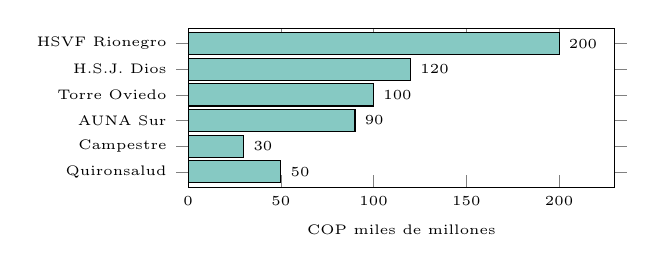
\begin{tikzpicture}
\begin{axis}[
  width=7cm, height=3.6cm,
  xbar, bar width=8pt,
  xlabel={\tiny COP miles de millones},
  symbolic y coords={Quironsalud,Campestre,AUNA Sur,Torre Oviedo,H.S.J. Dios,HSVF Rionegro},
  ytick=data,
  yticklabel style={font=\tiny},
  xticklabel style={font=\tiny},
  xmin=0, xmax=230,
  clip=false,
  nodes near coords={\tiny\pgfmathprintnumber\pgfplotspointmeta},
  nodes near coords align={horizontal},
  grid=none,
  enlarge y limits=0.12,
]
\addplot[fill=teal!50] coordinates {
  (200,HSVF Rionegro)
  (120,H.S.J. Dios)
  (100,Torre Oviedo)
  (90,AUNA Sur)
  (30,Campestre)
  (50,Quironsalud)
};
\end{axis}
\end{tikzpicture}

\src{Prensa verificada, REPS, estados financieros}

\column{0.47\textwidth}
\vspace{2pt}
\begin{alertblock}{\small Señal del mercado}
\scriptsize
\textbf{6 instituciones} invirtiendo en el corredor:

\vspace{2pt}
\begin{itemize}\setlength{\itemsep}{1pt}
  \item HSVF Rionegro: expansión a \textbf{500 camas}
  \item Torre Oviedo: \textbf{87 consultorios} (jun 2025)
  \item AUNA Sur: \textbf{168 camas} Envigado
  \item Campestre: \textbf{sede Rionegro} (mar 2026, 250 pac/día)
\end{itemize}
\end{alertblock}

\vspace{2pt}
{\scriptsize Ventana de oportunidad: \danger{2026--2028}. Nicho ambulatorio premium será ocupado si HPTU no actúa.}

\vspace{2pt}
\begin{exampleblock}{\small Respuesta}
\centering\normalsize
\highlight{Sí. COP \$590,000M.}
\end{exampleblock}
\end{columns}
\end{frame}

% ---- SLIDE 17: Q5 DETALLE — COMPETIDORES ----
\begin{frame}{Paisaje competitivo: 13 instituciones perfiladas}

\vspace{-4pt}
{\tiny\setlength{\tabcolsep}{3pt}
\begin{tabular}{@{}lrcllll@{}}
\toprule
\textbf{Institución} & \textbf{Camas} & \textbf{UCI} & \textbf{Ubicación} & \textbf{Complejidad} & \textbf{Movimiento reciente} & \textbf{Amenaza} \\
\midrule
\rowcolor{coral!8}
HSVF Rionegro & 152 & --- & Rionegro & alta & Exp.\ 500 camas, helipuerto & \danger{ALTA} \\
\rowcolor{coral!8}
Cl.\ Somer & 200 & 19 & Rionegro & alta & Trasplante cardíaco, oncol.\ ped. & \danger{ALTA} \\
\rowcolor{coral!6}
Cl.\ Rosario Tesoro & 140 & 60 & El Poblado & alta & Oncología integral & \danger{ALTA} \\
\rowcolor{coral!6}
Cl.\ del Campestre & --- & --- & Poblado + Rionegro & media-alta & Sede Rionegro mar 2026, 250 pac/día & \danger{ALTA} \\
HSVF Medellín & 525 & 208 & Centro & alta & Exp.\ quemados & MEDIA \\
AUNA (Main + Sur) & 492 & --- & Med + Envigado & alta & Sede Sur 168 camas & MEDIA \\
Quironsalud & 812 & --- & Varios & alta & Adquis.\ COA + Clofan & MEDIA \\
Torre Oviedo & --- & --- & El Poblado & media-alta & 87 consultorios, jun 2025 & MEDIA \\
Proy.\ Alto Palmas & --- & --- & Las Palmas & media & En evaluación & MEDIA \\
IPS Universitaria & 604 & 141 & Varios & alta & N/D & BAJA \\
CardioVID & 200 & --- & Medellín & alta & Planes exp. & BAJA \\
Cl.\ Vitha & 201 & 36 & Laureles & alta & Inaugurada 2024 & BAJA \\
H.\ San Juan Dios & --- & --- & Rionegro & media & Torre \$120,000M estudios & MEDIA \\
\bottomrule
\end{tabular}
}

\vspace{4pt}
\begin{columns}[T]
\column{0.48\textwidth}
{\scriptsize\textbf{4 amenaza ALTA}: todos en corredor sur-oriente. \textbf{Ninguno} ofrece alta complejidad tipo HPTU.}
\column{0.48\textwidth}
{\scriptsize\textbf{Oportunidad}: 10 categorías ambulatorias son \textbf{críticas o inexistentes} en el Oriente.}
\end{columns}
\end{frame}

% ---- SLIDE 18: Q6 TURISMO DE SALUD ----
\begin{frame}{Q6: ¿Hay potencial de turismo de salud?}

\begin{columns}[T]
\column{0.50\textwidth}
\vspace{4pt}
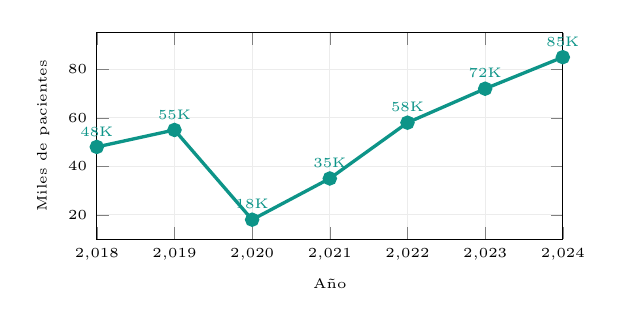
\begin{tikzpicture}
\begin{axis}[
  width=7.5cm, height=4.2cm,
  xlabel={\tiny Año},
  ylabel={\tiny Miles de pacientes},
  xmin=2018, xmax=2024,
  ymin=10, ymax=95,
  xtick={2018,2019,2020,2021,2022,2023,2024},
  xticklabel style={font=\tiny},
  yticklabel style={font=\tiny},
  grid=major, grid style={gray!15},
  nodes near coords={\tiny\pgfmathprintnumber\pgfplotspointmeta K},
  every node near coord/.append style={anchor=south},
]
\addplot[teal, very thick, mark=*, mark size=2pt] coordinates {
  (2018,48)(2019,55)(2020,18)(2021,35)(2022,58)(2023,72)(2024,85)
};
\end{axis}
\end{tikzpicture}

\vspace{2pt}
\src{ProColombia, DANE EVI, SISPRO}

\vspace{4pt}
{\scriptsize Top orígenes: EEUU (50.5\%), Panamá (16.7\%), Aruba (7.7\%), Col.\ residentes exterior (4.0\%)}

\column{0.47\textwidth}
\vspace{4pt}
{\small 3 KPIs del turismo médico:}

\vspace{6pt}
\begin{exampleblock}{}
\centering
{\Large \highlight{85,000}} \\
\footnotesize pacientes/año (2024)
\end{exampleblock}

\vspace{2pt}
\begin{exampleblock}{}
\centering
{\Large \highlight{USD \$235M}} \\
\footnotesize revenue anual
\end{exampleblock}

\vspace{2pt}
\begin{exampleblock}{}
\centering
{\Large \highlight{+11.9\%}} \\
\footnotesize crecimiento YoY
\end{exampleblock}

\vspace{4pt}
{\footnotesize Gasto promedio: \textbf{USD \$2,764} por visita. Estadía promedio: \textbf{14.2 noches}.}
\end{columns}
\end{frame}

% ---- SLIDE 19: Q6 DETALLE — VENTAJA JCI ----
\begin{frame}{Ventaja JCI: HPTU es el único en Antioquia}

\begin{columns}[T]
\column{0.46\textwidth}
\vspace{2pt}
{\footnotesize\textbf{Acreditación hospitalaria en Antioquia:}}

\vspace{4pt}
{\tiny
\begin{tabular}{@{}lllcc@{}}
\toprule
\textbf{Hospital} & \textbf{Ciudad} & \textbf{Acred.} & \textbf{Rating} & \textbf{$<$30' SKRG} \\
\midrule
\rowcolor{teal!12}
\textbf{HPTU} & Medellín & \highlight{JCI} & \textbf{4.4} & \danger{No} \\
Cl.\ Somer & Rionegro & BPC & 3.7 & Sí \\
HSVF Rionegro & Rionegro & BPC & --- & Sí \\
Cl.\ El Rosario & Medellín & BPC & 3.3 & No \\
Cl.\ Las Americas & Medellín & BPC & 3.7 & No \\
CardioVID & Medellín & BPC & --- & No \\
\bottomrule
\end{tabular}
}

\vspace{3pt}
{\scriptsize JCI = Joint Commission International. Solo \textbf{6 JCI} en Colombia. HPTU es el \textbf{único en Antioquia}.}

\src{REPS BPC, JCI Directory, Google Places}

\column{0.51\textwidth}
\vspace{2pt}
\begin{alertblock}{\small El dato clave}
\scriptsize
\danger{0 instituciones JCI} a menos de 30 min del Aeropuerto SKRG.

\vspace{3pt}
HPTU campus: \textbf{57 min} al aeropuerto.\\
Access Point Km 7 (vía Túnel): \highlight{25 min}. Reducción: \highlight{--32 min}.
\end{alertblock}

\vspace{4pt}
\begin{exampleblock}{\small Captura potencial}
\footnotesize
Si Km 7 captura solo \textbf{5\%} del turismo médico:

\vspace{3pt}
\centering
4,250 pac/año $\times$ USD \$2,764\\
= \highlight{USD \$11.7M adicionales/año}
\end{exampleblock}

\vspace{4pt}
\begin{exampleblock}{\small Respuesta}
\centering\large
\highlight{Sí. USD \$11.7M.}
\end{exampleblock}
\end{columns}
\end{frame}

% ---- SLIDE 20: RESUMEN 6 PREGUNTAS ----
{
\setbeamercolor{background canvas}{bg=teal!3}
\begin{frame}{6 preguntas, 6 respuestas: todas Sí}

\begin{center}
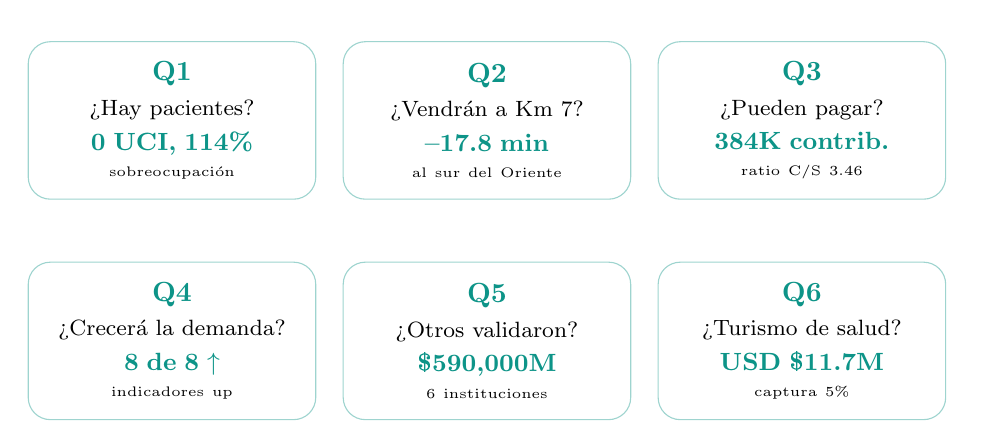
\begin{tikzpicture}[
  qbox/.style={draw=teal!40, fill=white, rounded corners=8pt,
               text width=3.3cm, minimum height=2.0cm, align=center,
               font=\footnotesize, inner sep=5pt},
  qlabel/.style={font=\tiny\bfseries, teal},
]
\node[qbox] (q1) at (0,0) {
  {\normalsize\textcolor{teal}{\textbf{Q1}}}\\[3pt]
  ¿Hay pacientes?\\[3pt]
  {\small\highlight{0 UCI, 114\%}}\\{\tiny sobreocupación}
};
\node[qbox] (q2) at (4,0) {
  {\normalsize\textcolor{teal}{\textbf{Q2}}}\\[3pt]
  ¿Vendrán a Km 7?\\[3pt]
  {\small\highlight{--17.8 min}}\\{\tiny al sur del Oriente}
};
\node[qbox] (q3) at (8,0) {
  {\normalsize\textcolor{teal}{\textbf{Q3}}}\\[3pt]
  ¿Pueden pagar?\\[3pt]
  {\small\highlight{384K contrib.}}\\{\tiny ratio C/S 3.46}
};
\node[qbox] (q4) at (0,-2.8) {
  {\normalsize\textcolor{teal}{\textbf{Q4}}}\\[3pt]
  ¿Crecerá la demanda?\\[3pt]
  {\small\highlight{8 de 8 $\uparrow$}}\\{\tiny indicadores up}
};
\node[qbox] (q5) at (4,-2.8) {
  {\normalsize\textcolor{teal}{\textbf{Q5}}}\\[3pt]
  ¿Otros validaron?\\[3pt]
  {\small\highlight{\$590,000M}}\\{\tiny 6 instituciones}
};
\node[qbox] (q6) at (8,-2.8) {
  {\normalsize\textcolor{teal}{\textbf{Q6}}}\\[3pt]
  ¿Turismo de salud?\\[3pt]
  {\small\highlight{USD \$11.7M}}\\{\tiny captura 5\%}
};

% Checkmarks
\foreach \q in {q1,q2,q3,q4,q5,q6} {
  \node[font=\large, teal, above right=-2pt and -2pt of \q.north east] {\checkmark};
}
\end{tikzpicture}
\end{center}

\vspace{6pt}
\begin{center}
{\large La demanda está \textbf{validada por 6 dimensiones independientes}. El riesgo no es invertir --- es \danger{no actuar}.}
\end{center}
\end{frame}
}

% ============================================================
% ACTO 4: ANÁLISIS Y RECOMENDACIÓN (slides 21--27, ~12 min)
% ============================================================

% ---- SLIDE 21: BRECHAS AMBULATORIAS ----
\begin{frame}{Brechas ambulatorias en el Oriente: 10 servicios críticos}

{\scriptsize
\begin{tabular}{@{}p{3.2cm}p{2.8cm}lp{4.2cm}@{}}
\toprule
\textbf{Servicio} & \textbf{Status Oriente} & \textbf{Nivel} & \textbf{Oportunidad HPTU} \\
\midrule
\rowcolor{coral!10}
Cirugía Ambulat.\ Avanzada & Solo Campestre (recién) & \danger{Crítico} & Hub quirúrgico: ortopedia, urología, ORL \\
\rowcolor{coral!10}
Oncología Ambulatoria & Solo Somer (única UFCA) & \danger{Crítico} & Quimioterapia, segunda opinión \\
\rowcolor{coral!10}
Radioterapia & Solo Somer (único equipo) & \danger{Crítico} & Segundo centro de radioterapia \\
Imágenes Avanzadas & IMEDI + Somer (limitado) & Limitado & TAC, RMN, PET-CT \\
\rowcolor{coral!6}
Rehabilitación Especial. & Básica únicamente & \danger{Inexist.} & Neuro-rehab, cardíaca, deportiva \\
\rowcolor{coral!6}
Chequeo Ejecutivo & Inexistente & \danger{Inexist.} & Check-up para ZF + aeropuerto \\
\rowcolor{coral!6}
Turismo Médico & 0 infraestructura & \danger{Inexist.} & 23,323 pac/año, 0 cerca SKRG \\
\rowcolor{coral!6}
Pediatría Subespec. & En Medellín & \danger{Inexist.} & Consulta pediátrica ambulatoria \\
Hemodiálisis & RCS Rionegro (41\%) & Limitado & Expansión puntos de diálisis \\
Cardiología Interv. & Solo Somer Incare & Limitado & 2do centro cardiovascular \\
\bottomrule
\end{tabular}
}

\vspace{4pt}
{\footnotesize \textbf{3 críticos + 4 inexistentes} = oportunidad masiva para hub ambulatorio especializado.}
\end{frame}

% ---- SLIDE 22: MCDA 6 ZONAS ----
\begin{frame}{MCDA: 6 zonas evaluadas --- el ranking}

\begin{center}
{\small Modelo MCDA: Accesibilidad (35\%) + Demanda (30\%) + Competencia (20\%) + Valor Inmobiliario (15\%)}
\end{center}

\vspace{6pt}
\begin{center}
{\small
\begin{tabular}{@{}lcccccc@{}}
\toprule
\textbf{Zona candidata} & \textbf{Acc.} & \textbf{Dem.} & \textbf{Comp.} & \textbf{Valor} & \textbf{SCORE} & \textbf{min a HPTU} \\
\midrule
\rowcolor{teal!12}
\textbf{Las Palmas Bajo} & \textbf{92} & \textbf{93} & \textbf{78} & \textbf{80} & \highlight{88} & 23.8 \\
\rowcolor{coral!4}
Access Point Km 7 & 85 & 91 & 65 & 75 & \textbf{81} & 18.5 \\
Las Palmas Medio & 72 & 84 & 82 & 70 & 77 & 31.8 \\
Envigado--Zúñiga & 75 & 80 & 62 & 74 & 74 & 22.4 \\
N.\ Poblado--Itagüí & 82 & 68 & 52 & 58 & 67 & 19.0 \\
\rowcolor{coral!6}
Las Palmas Alto & 42 & 52 & 90 & 62 & \danger{58} & 57.1 \\
\bottomrule
\end{tabular}
}
\end{center}

\vspace{6pt}
\begin{columns}[T]
\column{0.32\textwidth}
\begin{block}{\small \#1 LP Bajo (88)}
\footnotesize Score más alto en MCDA. POT 9/9.
\end{block}

\column{0.32\textwidth}
\begin{exampleblock}{\small \#2 Access Point (81)}
\footnotesize \highlight{Recomendado}: demanda dual Poblado + 460K Oriente + aeropuerto.
\end{exampleblock}

\column{0.32\textwidth}
\begin{alertblock}{\small \#6 LP Alto (58)}
\footnotesize \danger{Descartado}: 57 min a HPTU, suelo rural. Inviable.
\end{alertblock}
\end{columns}
\end{frame}

% ---- SLIDE 23: ACCESS POINT KM 7 ----
\begin{frame}{Access Point Km 7: nuestra recomendación estratégica}

\begin{columns}[T]
\column{0.46\textwidth}
\vspace{-2pt}
{\scriptsize\setlength{\tabcolsep}{3pt}
\begin{tabular}{@{}ll@{}}
\toprule
Score MCDA & \highlight{81/100} (\#2 --- decisión estratégica \#1) \\
Ubicación & Km 7 Vía Las Palmas, Retorno 5 \\
Infraestructura & 4 torres, 10 pisos, 1,085 parq. \\
A HPTU actual & 18.5 min \\
A Aeropuerto & \highlight{25 min} (vía Túnel H2 2027) \\
A Rionegro & \highlight{25 min} (post doble calzada) \\
Pico y placa & \highlight{Sin restricción} \\
\bottomrule
\end{tabular}
}

\vspace{6pt}
{\small\textbf{Catchment dual:}}

\vspace{3pt}
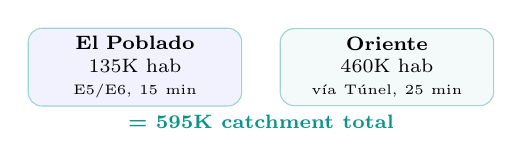
\begin{tikzpicture}[
  catch/.style={draw=teal!40, fill=white, rounded corners=5pt,
                text width=2.5cm, minimum height=0.9cm, align=center,
                font=\scriptsize, inner sep=3pt},
]
\node[catch, fill=blue!5] (c1) at (0,0) {
  \textbf{El Poblado}\\135K hab\\{\tiny E5/E6, 15 min}
};
\node[catch, fill=teal!5] (c2) at (3.2,0) {
  \textbf{Oriente}\\460K hab\\{\tiny vía Túnel, 25 min}
};
\node[font=\scriptsize\bfseries, teal] at (1.6, -0.7) {= \highlight{595K} catchment total};
\end{tikzpicture}

\column{0.50\textwidth}
\vspace{-2pt}
{\small\textbf{Nodo estratégico del Túnel:}}

\vspace{4pt}
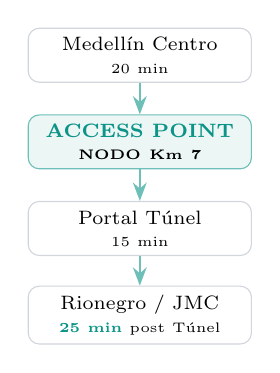
\begin{tikzpicture}[
  node distance=0.3cm,
  stop/.style={draw=slate!30, fill=white, rounded corners=4pt,
               text width=2.6cm, minimum height=0.6cm, align=center,
               font=\scriptsize},
  hub/.style={stop, draw=teal!60, fill=teal!8, font=\scriptsize\bfseries},
]
\node[stop] (med) at (0,0) {Medellín Centro\\{\tiny 20 min}};
\node[hub] (ap) at (0,-1.1) {\textcolor{teal}{ACCESS POINT}\\{\tiny NODO Km 7}};
\node[stop] (tunel) at (0,-2.2) {Portal Túnel\\{\tiny 15 min}};
\node[stop] (rio) at (0,-3.3) {Rionegro / JMC\\{\tiny \highlight{25 min} post Túnel}};

\draw[-{Stealth}, thick, teal!60] (med) -- (ap);
\draw[-{Stealth}, thick, teal!60] (ap) -- (tunel);
\draw[-{Stealth}, thick, teal!60] (tunel) -- (rio);
\end{tikzpicture}

\vspace{4pt}
\begin{exampleblock}{\small Por qué es la recomendación}
\scriptsize
Único punto que conecta \textbf{dos mercados} simultáneamente: El Poblado (135K, E5/E6) y todo el Oriente (460K, 384K contributivos). Post Túnel, \textbf{ningún destino queda a más de 40 min}.
\end{exampleblock}
\end{columns}
\end{frame}

% ---- SLIDE ~: POR QUÉ RECOMENDAMOS ACCESS POINT ----
{
\setbeamercolor{background canvas}{bg=teal!3}
\begin{frame}{Score \#2, decisión \#1: ¿por qué Access Point?}

\vspace{-2pt}
\begin{columns}[T]
\column{0.46\textwidth}
{\scriptsize\setlength{\tabcolsep}{3pt}
\begin{tabular}{@{}lcccc@{}}
\toprule
\textbf{Dimensión} & \textbf{Peso} & \textbf{LP Bajo} & \textbf{AP Km 7} & \textbf{$\Delta$} \\
\midrule
\rowcolor{teal!6}
Accesibilidad & 35\% & 92 & 85 & +7 \\
Demanda & 30\% & 93 & 91 & +2 \\
\rowcolor{coral!6}
Competencia & 20\% & 78 & 65 & +13 \\
Valor Inmob. & 15\% & 80 & 75 & +5 \\
\midrule
\textbf{TOTAL} & & \textbf{88} & \textbf{81} & +7 \\
\bottomrule
\end{tabular}
}

\vspace{3pt}
{\scriptsize Diferencia: \textbf{competencia} (40+ IPS en 5 km de AP). Pero \textbf{ninguna} ofrece trasplantes, hematología ni JCI.}

\vspace{3pt}
\begin{block}{\small Lo que el MCDA no captura}
\scriptsize
El modelo evalúa \textbf{hoy}. No pondera la transformación que viene: Túnel doble calzada, Oriente creciendo al doble, aeropuerto triplicando.
\end{block}

\column{0.50\textwidth}
\vspace{-2pt}
\begin{exampleblock}{\small 6 razones estratégicas}
\scriptsize
\begin{enumerate}\setlength{\itemsep}{1pt}\setlength{\parskip}{0pt}
  \item \textbf{595K} catchment dual (Poblado + Oriente)
  \item \textbf{25 min} al aeropuerto (vía Túnel) --- JCI
  \item \textbf{45K consultas/año} capturable del Oriente
  \item \textbf{Infraestructura lista}: 4 torres, 1,085 parq.
  \item \textbf{Nodo Túnel}: Rionegro a 25 min (H2 2027)
  \item \textbf{Oriente +2\%} anual vs Medellín +0.9\%
\end{enumerate}
\end{exampleblock}
\end{columns}

\vspace{4pt}
\begin{alertblock}{\small Nuestra recomendación}
\scriptsize
El MCDA sitúa a LP Bajo como \#1 en condiciones actuales. Pero la inversión mira a \textbf{10--15 años}. Los fundamentales del Oriente --- 728K hab., +2\% CAGR, 384K contributivos, aeropuerto triplicando, Túnel doble calzada --- hacen de Access Point la \textbf{posición estratégica superior}. \highlight{Recomendamos Access Point Km 7.}
\end{alertblock}
\end{frame}
}

% ---- SLIDE ~: ISOCRONAS ----
\begin{frame}{Isocronas de accesibilidad: ¿quién llega en cuánto tiempo?}

\begin{columns}[T]
\column{0.48\textwidth}
\vspace{4pt}
{\small\textbf{Desde Access Point Km 7} (Mapbox Isochrone):}

\vspace{6pt}
{\scriptsize
\begin{tabular}{@{}lp{5cm}@{}}
\toprule
\textbf{Isocrona} & \textbf{Cobertura} \\
\midrule
\rowcolor{teal!10}
\textbf{15 min} & El Poblado sur, El Tesoro, San Lucas, Altos del Poblado \\
\textbf{20 min} & Milla de Oro, Envigado norte, Club El Rodeo \\
\rowcolor{teal!6}
\textbf{30 min} & Todo El Poblado, Envigado, Laureles, acceso Túnel Oriente \\
\textbf{45 min} & El Retiro, Guarne, acceso aeropuerto \\
\rowcolor{amber!8}
\textbf{60 min} & Rionegro, La Ceja, Marinilla, aeropuerto SKRG \\
\bottomrule
\end{tabular}
}

\vspace{4pt}
{\footnotesize \highlight{135K habitantes} en 15 min + \highlight{460K Oriente} en 45--60 min.}

\column{0.49\textwidth}
\vspace{4pt}
{\small\textbf{Post Túnel doble calzada} (H2 2027):}

\vspace{6pt}
{\scriptsize
\begin{tabular}{@{}lcccc@{}}
\toprule
\textbf{Destino} & \textbf{Km 7} & \textbf{Post Túnel} & \textbf{HPTU} & \textbf{$\Delta$} \\
\midrule
\rowcolor{teal!8}
Aeropuerto & 51' & \highlight{25'} & 66' & \highlight{--41'} \\
\rowcolor{teal!8}
Rionegro & 59' & \highlight{25'} & 57' & \highlight{--32'} \\
El Retiro & 44' & \highlight{30'} & 62' & \highlight{--32'} \\
El Poblado & 10' & 10' & 24' & --14' \\
\rowcolor{teal!6}
La Ceja & 66' & \highlight{40'} & 84' & \highlight{--44'} \\
\bottomrule
\end{tabular}
}

\vspace{6pt}
{\footnotesize Post Túnel, Km 7 gana en \textbf{todos los destinos} --- incluyendo Rionegro donde hoy empata con HPTU.}
\end{columns}
\end{frame}

% ---- SLIDE 25: CONVERGENCIA ----
{
\setbeamercolor{background canvas}{bg=teal!3}
\begin{frame}{Convergencia de evidencia: 5 pilares}

\begin{center}
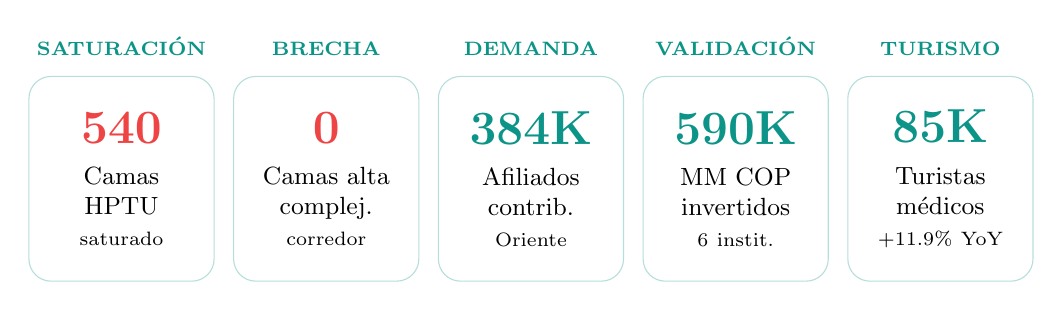
\begin{tikzpicture}[
  pillar/.style={draw=teal!30, fill=white, rounded corners=8pt,
                 text width=2.0cm, minimum height=2.6cm, align=center,
                 font=\small, inner sep=5pt},
  plabel/.style={font=\scriptsize\bfseries, teal},
]
\node[pillar] (p1) at (0,0) {
  {\LARGE\textcolor{coral}{\textbf{540}}}\\[4pt]
  Camas\\HPTU\\{\scriptsize saturado}
};
\node[pillar] (p2) at (2.6,0) {
  {\LARGE\textcolor{coral}{\textbf{0}}}\\[4pt]
  Camas alta\\complej.\\{\scriptsize corredor}
};
\node[pillar] (p3) at (5.2,0) {
  {\LARGE\textcolor{teal}{\textbf{384K}}}\\[4pt]
  Afiliados\\contrib.\\{\scriptsize Oriente}
};
\node[pillar] (p4) at (7.8,0) {
  {\LARGE\textcolor{teal}{\textbf{590K}}}\\[4pt]
  MM COP\\invertidos\\{\scriptsize 6 instit.}
};
\node[pillar] (p5) at (10.4,0) {
  {\LARGE\textcolor{teal}{\textbf{85K}}}\\[4pt]
  Turistas\\médicos\\{\scriptsize +11.9\% YoY}
};

\node[plabel, above=4pt of p1] {SATURACIÓN};
\node[plabel, above=4pt of p2] {BRECHA};
\node[plabel, above=4pt of p3] {DEMANDA};
\node[plabel, above=4pt of p4] {VALIDACIÓN};
\node[plabel, above=4pt of p5] {TURISMO};
\end{tikzpicture}
\end{center}

\vspace{10pt}
{\normalsize Cada pilar por separado justifica la exploración. \textbf{Los 5 juntos} constituyen el caso más sólido para expansión estratégica del HPTU.}

\vspace{6pt}
{\footnotesize No encontramos un solo indicador que contradiga la tesis. \textbf{La evidencia es unánime.}}
\end{frame}
}

% ---- SLIDE 26: RECOMENDACIÓN ----
{
\setbeamercolor{background canvas}{bg=teal!3}
\begin{frame}{Recomendación: Access Point Km 7 --- Posición estratégica}

\begin{columns}[T]
\column{0.42\textwidth}
\textbf{Ubicación}: Km 7 Vía Las Palmas, Retorno 5\\
{\footnotesize Acierto Inmobiliario --- nodo de entrada al Túnel}

\vspace{6pt}
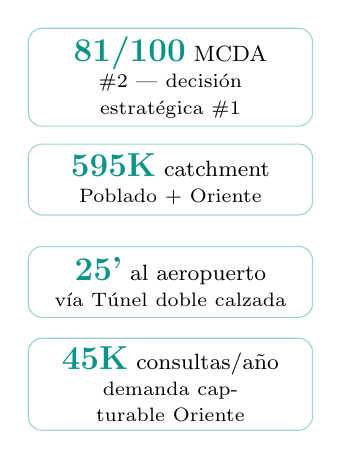
\begin{tikzpicture}[
  pillar/.style={draw=teal!40, fill=white, rounded corners=5pt,
                 text width=3.4cm, minimum height=0.9cm, align=center,
                 font=\footnotesize, inner sep=3pt},
]
\node[pillar] (p1) at (0,0) {
  {\large\textcolor{teal}{\textbf{81/100}}} MCDA\\{\scriptsize \#2 --- decisión estratégica \#1}
};
\node[pillar] (p2) at (0,-1.3) {
  {\large\textcolor{teal}{\textbf{595K}}} catchment\\{\scriptsize Poblado + Oriente}
};
\node[pillar] (p3) at (0,-2.6) {
  {\large\textcolor{teal}{\textbf{25'}}} al aeropuerto\\{\scriptsize vía Túnel doble calzada}
};
\node[pillar] (p4) at (0,-3.9) {
  {\large\textcolor{teal}{\textbf{45K}}} consultas/año\\{\scriptsize demanda capturable Oriente}
};
\end{tikzpicture}

\column{0.55\textwidth}
{\footnotesize
\begin{tabular}{@{}p{3.8cm}l@{}}
\toprule
\textbf{Parámetro} & \textbf{Valor} \\
\midrule
Infraestructura & 4 torres, 10 pisos \\
Parqueaderos & \highlight{1,085} \\
A HPTU actual & 18.5 min \\
A Aeropuerto (vía Túnel) & \highlight{25 min} \\
Catchment dual & \highlight{135K + 460K = 595K} \\
Pico y placa & Sin restricción \\
Post Túnel: Rionegro & \highlight{25 min} \\
\bottomrule
\end{tabular}
}

\vspace{6pt}
\begin{exampleblock}{\small ¿Por qué AP sobre LP Bajo?}
\scriptsize LP Bajo tiene score 88 (\#1 en MCDA). Pero la inversión mira a \textbf{10--15 años}. Los fundamentales del Oriente --- \highlight{728K hab}, crecimiento +2\% anual, \highlight{384K contributivos}, aeropuerto triplicando, Túnel doble calzada --- hacen de AP la \textbf{posición de mayor valor prospectivo}.
\end{exampleblock}
\end{columns}
\end{frame}
}

% ---- SLIDE 27: MODELO FINANCIERO ----
\begin{frame}{Modelo financiero: factibilidad por zona}

\begin{columns}[T]
\column{0.46\textwidth}
{\scriptsize
\begin{tabular}{@{}l r r r r@{}}
\toprule
\textbf{Zona} & \textbf{Camas} & \textbf{Inv.} & \textbf{Payb.} & \textbf{VPN} \\
\midrule
\rowcolor{teal!10}
\textbf{LP Bajo} & \textbf{250} & \textbf{\$90MM} & \textbf{11.3y} & \highlight{+\$4.8} \\
LP Medio & 300 & \$108MM & 9.4y & +\$15.3 \\
Envigado & 220 & \$82MM & 11.3y & +\$4.0 \\
N.\ Poblado & 260 & \$98MM & 9.6y & +\$14.7 \\
\rowcolor{coral!8}
LP Alto & 150 & \$55MM & \danger{22.9y} & \danger{--\$31} \\
\bottomrule
\end{tabular}
}
{\tiny Miles de MM COP. WACC 12\%, ramp-up 60\%/80\%/100\%.}

\vspace{4pt}
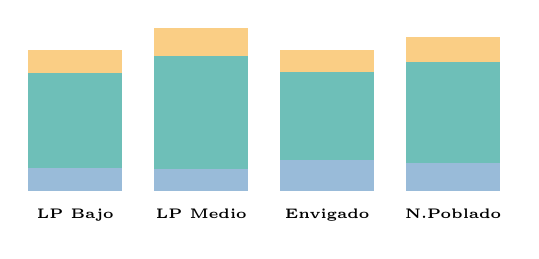
\begin{tikzpicture}
  \foreach \x/\label/\land/\const/\equip in {
    0/LP Bajo/15/60/15,
    1.6/LP Medio/14/72/18,
    3.2/Envigado/20/56/14,
    4.8/N.Poblado/18/64/16} {
    \pgfmathsetmacro{\landh}{\land/90*1.8}
    \pgfmathsetmacro{\consth}{\const/90*1.8}
    \pgfmathsetmacro{\equiph}{\equip/90*1.8}
    \fill[hptu!40] (\x,0) rectangle (\x+1.2, \landh);
    \fill[teal!60] (\x,\landh) rectangle (\x+1.2, \landh+\consth);
    \fill[amber!50] (\x,\landh+\consth) rectangle (\x+1.2, \landh+\consth+\equiph);
    \node[font=\tiny\bfseries, below] at (\x+0.6, -0.1) {\label};
  }
\end{tikzpicture}

\column{0.50\textwidth}
\begin{block}{\small Parámetros base}
\tiny
\begin{tabular}{@{}ll@{}}
Construcción/m² & \$4.0M (Scielo/U.\ Militar) \\
Dotación & 25\% (DNP) \\
Ocupación & 80\% (estándar) \\
Ingreso/cama/año & \$1,600M (HUSI) {\color{coral}$\blacktriangledown$} \\
EBITDA & 8\% {\color{coral}$\blacktriangledown$} \\
WACC & 12\% {\color{coral}$\blacktriangledown$} \\
\end{tabular}
\end{block}

\vspace{4pt}
\begin{exampleblock}{\small Sensibilidad}
\footnotesize Si ingreso/cama = \$2,000M (privado premium):

\vspace{3pt}
VPN LP Bajo: \highlight{+\$4.8MM $\to$ +\$25MM}

\vspace{3pt}
Este es el parámetro \textbf{más sensible} del modelo.
\end{exampleblock}
\end{columns}
\end{frame}

% ============================================================
% ACTO 5: DECISIÓN (slides 28--33, ~10 min + Q&A)
% ============================================================

% ---- SLIDE 28: VIABILIDAD POT ----
\begin{frame}{Viabilidad POT: 22 barrios, Altos del Poblado líder}

\begin{columns}[T]
\column{0.50\textwidth}
{\scriptsize
\begin{tabular}{@{}lcccr@{}}
\toprule
\textbf{Barrio} & \textbf{Score} & \textbf{CL\_D} & \textbf{Pisos} & \textbf{Suelo (m²)} \\
\midrule
\rowcolor{teal!10}
\textbf{Altos del Poblado} & \highlight{9/9} & 2.38 & 11.7 & 68,020 \\
\rowcolor{teal!6}
El Tesoro & 9/9 & 2.52 & 7.2 & 119,482 \\
Castropol & 8/9 & 1.89 & 7.1 & 65,591 \\
Los Balsos No.\ 1 & 8/9 & 2.15 & 11.5 & 97,440 \\
\midrule
Los Balsos No.\ 2 & 6/9 & & 16.7 & 132,161 \\
Las Lomas No.\ 1 & 5/9 & & 15.4 & 30,281 \\
Las Lomas No.\ 2 & 5/9 & & 20.0 & --- \\
\midrule
{\tiny + 15 barrios más} & 1--7 & & & \\
\bottomrule
\end{tabular}
}

\src{POT Batería Indicadores (3ciz-tpgr), Acuerdo 48 de 2014}

\vspace{4pt}
{\footnotesize CL\_D = Carga Localizada Dotacional. Valores $>$2.0 = aptos para uso dotacional de salud.}

\column{0.47\textwidth}
\begin{exampleblock}{\small Altos del Poblado: máxima viabilidad}
\footnotesize
\begin{itemize}
  \item CL\_D = \highlight{2.38}
  \item ICS = 57.4 (capacidad de soporte)
  \item ICF = 2.78 (flujos favorable)
  \item Suelo: \highlight{68,020 m²}
  \item Altura: 11.7 pisos (250 camas)
\end{itemize}
\end{exampleblock}

\vspace{4pt}
\begin{block}{\small Viabilidad por categoría}
\footnotesize
\begin{tabular}{@{}lcl@{}}
\textcolor{green}{$\bullet$} & ALTA (8--9) & 4 barrios \\
\textcolor{teal}{$\bullet$} & MEDIA-ALTA (6--7) & 6 barrios \\
\textcolor{amber}{$\bullet$} & MEDIA (4--5) & 7 barrios \\
\textcolor{coral}{$\bullet$} & BAJA (1--3) & 5 barrios \\
\end{tabular}
\end{block}

\vspace{4pt}
{\footnotesize\textcolor{coral}{$\blacktriangledown$} Pendiente: fichas normativas \textbf{por polígono} (DAP Medellín).}
\end{columns}
\end{frame}

% ---- SLIDE 29: LO QUE FALTA ----
{
\setbeamercolor{background canvas}{bg=coral!3}
\begin{frame}{Lo que falta: 8 parámetros por validar}

\vspace{-2pt}
{\scriptsize
\begin{tabular}{@{}p{4.0cm}ccl@{}}
\toprule
\textbf{Parámetro} & \textbf{Prior.} & \textbf{Valor actual} & \textbf{Fuente de validación} \\
\midrule
\rowcolor{coral!8}
Precio suelo/m² por zona & \danger{ALTA} & \$0.5--2.5M/m² & Lonja de Propiedad Raíz \\
\rowcolor{coral!8}
Ingreso/cama/año & \danger{ALTA} & \$1,600M COP & Pablo Tobón, Las Américas \\
\rowcolor{coral!6}
Margen EBITDA operativo & \danger{ALTA} & 8\% & Supersalud (EE.FF.) \\
Fichas normativas POT & \danger{ALTA} & Estimadas & DAP Medellín / GeoMedellín \\
Lotes disponibles & \danger{ALTA} & 8--15K m² & Inmobiliarias corredor \\
\rowcolor{amber!10}
WACC del proyecto & MEDIA & 12\% & Banca de inversión \\
\rowcolor{amber!10}
Costos diseño + licencias & MEDIA & 18 meses est. & Arquitectura hospitalaria \\
IO/IC específico por lote & MEDIA & Estimados & Fichas normativas POT \\
\bottomrule
\end{tabular}
}

\vspace{4pt}
\begin{columns}[T]
\column{0.48\textwidth}
\begin{alertblock}{\small Sensibilidad}
\scriptsize
{\scriptsize
\begin{tabular}{@{}lcc@{}}
\toprule
\textbf{Escenario} & \textbf{Ingreso/cama} & \textbf{VPN LP Bajo} \\
\midrule
\rowcolor{coral!6}
Conservador (HUSI) & \$1,600M & +\$4.8MM \\
\rowcolor{teal!6}
Privado premium & \$2,000M & \highlight{+\$25MM} \\
Privado alto & \$2,200M & +\$38MM \\
\bottomrule
\end{tabular}
}
\end{alertblock}

\column{0.48\textwidth}
\begin{block}{\small Riesgos identificados}
\footnotesize
\begin{enumerate}\scriptsize
  \item Demoras en licenciamiento POT
  \item Volatilidad costos de construcción
  \item Cartera EPS ($\sim$\$14B COP sector)
  \item Nuevos competidores en el corredor
  \item Cambios regulatorios
\end{enumerate}
\end{block}
\end{columns}
\end{frame}
}

% ---- SLIDE 30: RUTA A LA DECISIÓN ----
\begin{frame}{Ruta a la decisión: Fases 3 y 4}

\begin{columns}[T]
\column{0.50\textwidth}
\textbf{Fase 3 --- Profundización} {\small(en curso)}

\vspace{4pt}
\begin{enumerate}\footnotesize
  \item[\textcolor{teal}{1.}] \textbf{Validar modelo financiero}\\
    {\scriptsize Lonja, Supersalud, benchmark hospitales privados}
  \item[\textcolor{teal}{2.}] \textbf{Due diligence POT}\\
    {\scriptsize Fichas normativas específicas por polígono}
  \item[\textcolor{teal}{3.}] \textbf{Identificar lotes}\\
    {\scriptsize Búsqueda activa con inmobiliarias}
  \item[\textcolor{teal}{4.}] \textbf{Competencia detallada}\\
    {\scriptsize Servicios, tarifas por zona}
  \item[\textcolor{teal}{5.}] \textbf{Análisis de sensibilidad}\\
    {\scriptsize Escenarios sobre parámetros críticos}
\end{enumerate}

\vspace{6pt}
\textbf{Fase 4 --- Recomendación Final}

\vspace{4pt}
\begin{enumerate}\footnotesize
  \item[\textcolor{hptu}{1.}] Informe ejecutivo final
  \item[\textcolor{hptu}{2.}] Shortlist de 2--3 lotes
  \item[\textcolor{hptu}{3.}] Análisis de escenarios para decisión
\end{enumerate}

\column{0.47\textwidth}
\begin{block}{\small Entregables actuales}
\footnotesize
\begin{enumerate}
  \item \textbf{Plataforma web} interactiva\\
    {\scriptsize hptu-localizacion.vercel.app}
  \item \textbf{Dashboard de demanda} (6 preguntas)
  \item \textbf{Base georreferenciada} (15 GeoJSON)
  \item \textbf{Dashboard MCDA} (6 zonas)
  \item \textbf{Modelo financiero} preliminar
  \item \textbf{Perfiles de 13 competidores}
  \item \textbf{Análisis turismo de salud}
\end{enumerate}
\end{block}

\vspace{4pt}
\begin{exampleblock}{\small Referencia}
\footnotesize San Vicente Rionegro validó la expansión estratégica. Las Palmas Bajo sigue esa lógica: acercar alta complejidad al mercado E5/E6.
\end{exampleblock}
\end{columns}
\end{frame}

% ---- SLIDE 31: CRONOGRAMA ----
\begin{frame}{Cronograma propuesto: 6 semanas a la decisión}

\vspace{4pt}
\begin{center}
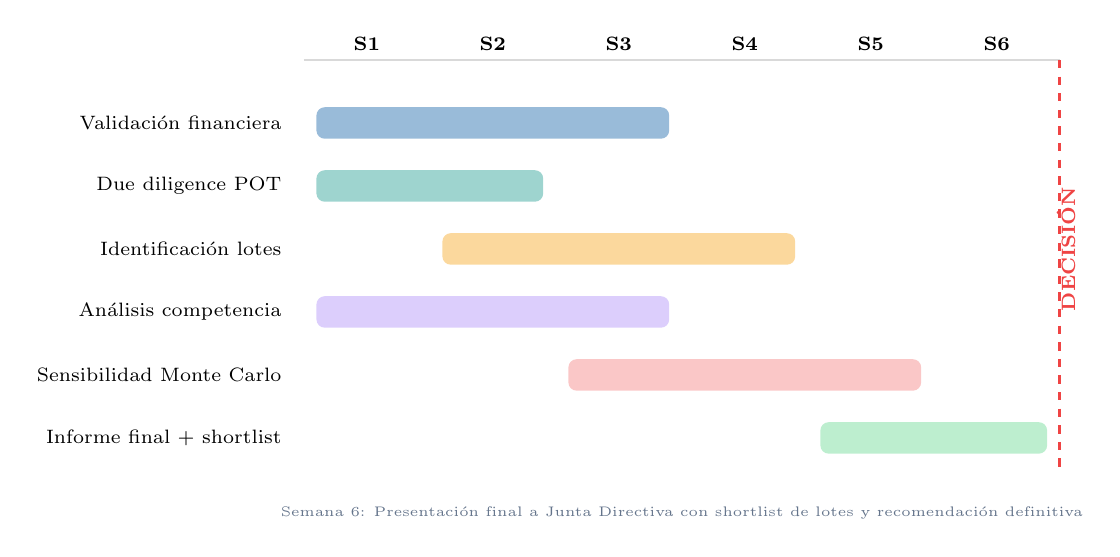
\begin{tikzpicture}[
  x=1.6cm, y=-0.8cm,
  task/.style={fill=#1, rounded corners=3pt, minimum height=0.5cm, inner sep=0pt},
]
% Header
\foreach \w/\label in {1/S1,2/S2,3/S3,4/S4,5/S5,6/S6} {
  \node[font=\scriptsize\bfseries, above] at (\w, 0) {\label};
}
\draw[gray!30] (0.5,0) -- (6.5,0);

% Tasks
\node[font=\scriptsize, anchor=east] at (0.4, 1) {Validación financiera};
\fill[hptu!40, rounded corners=3pt] (1-0.4, 0.75) rectangle (3+0.4, 1.25);

\node[font=\scriptsize, anchor=east] at (0.4, 2) {Due diligence POT};
\fill[teal!40, rounded corners=3pt] (1-0.4, 1.75) rectangle (2+0.4, 2.25);

\node[font=\scriptsize, anchor=east] at (0.4, 3) {Identificación lotes};
\fill[amber!40, rounded corners=3pt] (2-0.4, 2.75) rectangle (4+0.4, 3.25);

\node[font=\scriptsize, anchor=east] at (0.4, 4) {Análisis competencia};
\fill[violet!30, rounded corners=3pt] (1-0.4, 3.75) rectangle (3+0.4, 4.25);

\node[font=\scriptsize, anchor=east] at (0.4, 5) {Sensibilidad Monte Carlo};
\fill[coral!30, rounded corners=3pt] (3-0.4, 4.75) rectangle (5+0.4, 5.25);

\node[font=\scriptsize, anchor=east] at (0.4, 6) {Informe final + shortlist};
\fill[green!30, rounded corners=3pt] (5-0.4, 5.75) rectangle (6+0.4, 6.25);

% Milestone
\draw[coral, very thick, dashed] (6.5, 0) -- (6.5, 6.5);
\node[font=\scriptsize\bfseries, coral, rotate=90, anchor=south] at (6.7, 3) {DECISIÓN};

% Legend
\node[font=\tiny\color{slate}] at (3.5, 7.2) {Semana 6: Presentación final a Junta Directiva con shortlist de lotes y recomendación definitiva};
\end{tikzpicture}
\end{center}
\end{frame}

% ---- SLIDE 32: SÍNTESIS EJECUTIVA ----
{
\setbeamercolor{background canvas}{bg=hptu!3}
\begin{frame}{Síntesis ejecutiva}

\begin{center}
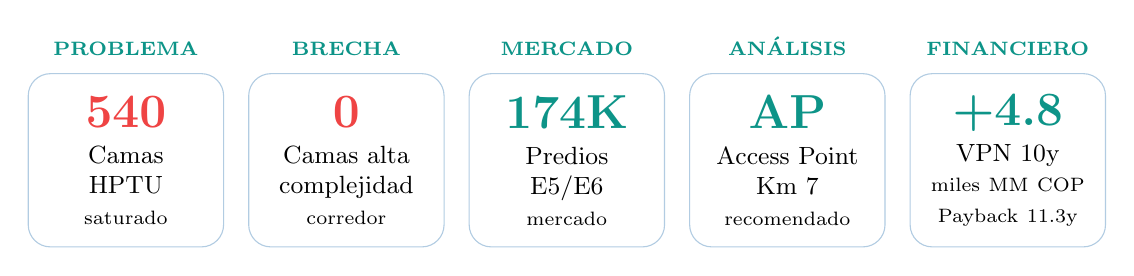
\begin{tikzpicture}[
  pillar/.style={draw=hptu!30, fill=white, rounded corners=8pt,
                 text width=2.2cm, minimum height=2.2cm, align=center,
                 font=\small, inner sep=4pt},
  plabel/.style={font=\scriptsize\bfseries, teal},
]
\node[pillar] (p1) at (0,0) {
  {\LARGE\textcolor{coral}{\textbf{540}}}\\[2pt]
  Camas\\HPTU\\{\scriptsize saturado}
};
\node[pillar] (p2) at (2.8,0) {
  {\LARGE\textcolor{coral}{\textbf{0}}}\\[2pt]
  Camas alta\\complejidad\\{\scriptsize corredor}
};
\node[pillar] (p3) at (5.6,0) {
  {\LARGE\textcolor{teal}{\textbf{174K}}}\\[2pt]
  Predios\\E5/E6\\{\scriptsize mercado}
};
\node[pillar] (p4) at (8.4,0) {
  {\LARGE\textcolor{teal}{\textbf{AP}}}\\[2pt]
  Access Point\\Km 7\\{\scriptsize recomendado}
};
\node[pillar] (p5) at (11.2,0) {
  {\LARGE\textcolor{teal}{\textbf{+4.8}}}\\[2pt]
  VPN 10y\\{\scriptsize miles MM COP}\\{\scriptsize Payback 11.3y}
};

\node[plabel, above=3pt of p1] {PROBLEMA};
\node[plabel, above=3pt of p2] {BRECHA};
\node[plabel, above=3pt of p3] {MERCADO};
\node[plabel, above=3pt of p4] {ANÁLISIS};
\node[plabel, above=3pt of p5] {FINANCIERO};
\end{tikzpicture}
\end{center}

\vspace{4pt}
\begin{columns}[T]
\column{0.48\textwidth}
\begin{exampleblock}{\small Lo que los datos dicen}
\scriptsize
\begin{enumerate}
  \item Sistema \textbf{saturado}, crecerá +152K personas
  \item Corredor: \textbf{0 camas} de alta complejidad
  \item \textbf{6 de 6 preguntas} respondidas con ``Sí''
  \item \textbf{Access Point Km 7}: posición estratégica para Oriente
  \item VPN positivo en \textbf{4 de 5 zonas}
\end{enumerate}
\end{exampleblock}

\column{0.48\textwidth}
\begin{alertblock}{\small La decisión pendiente}
\scriptsize Para pasar de recomendación a \textbf{decisión de inversión}:

\vspace{2pt}
\begin{enumerate}
  \item Validar 5 supuestos financieros
  \item Confirmar fichas normativas POT
  \item Identificar 2--3 lotes concretos
  \item Análisis de sensibilidad
\end{enumerate}

\vspace{1pt}
{\tiny 6 semanas a la decisión final.}
\end{alertblock}
\end{columns}
\end{frame}
}

% ---- SLIDE 33: CIERRE ----
{
\setbeamercolor{background canvas}{bg=hptu}
\begin{frame}[plain]
\vfill
\begin{center}
{\Huge\bfseries\textcolor{white}{¿Preguntas?}}

\vspace{20pt}
\begin{tikzpicture}
  \draw[white, line width=0.5pt] (0,0) -- (8,0);
\end{tikzpicture}

\vspace{16pt}
{\large\textcolor{white!90}{HPTU --- Nueva Sede}}

\vspace{6pt}
{\normalsize\textcolor{white!80}{Validación de Demanda y Localización Estratégica}}

\vspace{14pt}
{\small\textcolor{white!70}{Plataforma interactiva:}}\\
{\small\textcolor{white!90}{\url{https://hptu-localizacion.vercel.app}}}

\vspace{10pt}
{\small\textcolor{white!60}{15 fuentes oficiales $\cdot$ 3.8M+ registros $\cdot$ 6 preguntas respondidas}}

\vspace{6pt}
{\small\textcolor{white!60}{6 zonas evaluadas $\cdot$ 13 competidores $\cdot$ Modelo financiero preliminar}}

\vspace{20pt}
{\footnotesize\textcolor{white!40}{Todo es datos. Nada es opinión.}}
\end{center}
\begin{tikzpicture}[remember picture, overlay]
  \node[anchor=south]
    at ([yshift=14pt]current page.south) {
    
\includegraphics[height=1.2cm]{basica-white.png}
  };
\end{tikzpicture}
\vfill
\end{frame}
}

\end{document}
